%%%%%%%%%%%%%%%%%%%%%%%%%%%%%%%%%%%%%%%%%%%%%%%%%%%%%%%%%%%%%%%%%%%%%%%%%%%%%%
% University of Bristol presentation theme based on the PowerPoint template
%
% Copyright (c) 2012, 2020 David A.W. Barton (david.barton@bristol.ac.uk)
% All rights reserved.
%
% The latest version of this theme can be found at
%   https://github.com/db9052/UoB-beamer-theme
%
% This is dual licensed under the MIT license and CC BY 4.0
%%%%%%%%%%%%%%%%%%%%%%%%%%%%%%%%%%%%%%%%%%%%%%%%%%%%%%%%%%%%%%%%%%%%%%%%%%%%%%
% \documentclass[aspectratio=169, handout]{beamer}
\documentclass[aspectratio=169]{beamer}
    % Possible aspect ratios are 16:9, 16:10, 14:9, 5:4, 4:3 (default) and 3:2
    % (Remember to remove the colon, i.e., 16:9 becomes the option 169) 

\usetheme{UoB}
% If lualatex is used then Rockwell, Latin Modern math, and Arial are used as
% per the UoB style (you need these fonts installed; they are installed by 
% default on Windows). If pdflatex is used then Concrete, Euler math, and 
% Helvetica are used as the closest alternatives.

% To use the Rockwell font in Overleaf, you will need to download a copy of
% the Truetype font (various websites appear to have it available for free -
% licensing is uncertain though) and put it in this folder with the name
% "Rockwell.ttf" and then change the compiler (under the menu) to LuaLaTeX.

\bibliographystyle{apalike}


\usepackage{tikz}
%\usetikzlibrary{shapes,arrows,positioning}
\usetikzlibrary{automata,arrows,positioning,calc}
\usetikzlibrary{shapes,snakes}

\usepackage{amsmath}
\usepackage{amssymb}
\usepackage{dsfont}

\usepackage{mathtools}
\newcommand{\defeq}{\vcentcolon=}
\newcommand{\eqdef}{=\vcentcolon}
\newcommand{\Var}{\text{Var}}

\DeclareMathOperator*{\argmax}{argmax} % thin space, limits underneath in displays
\DeclareMathOperator*{\argmin}{argmin}

%%%%%%%%%%%%%%%%%%%%%%%%%%%%%%%%%%%%%%%%%%%%%%%%%%%%%%%%%%%%%%%%%%%%%%%%%%%%%%
\title[Short Title]{Self-Tuning Spectral Clustering}
% \subtitle{Filtering, Smoothing \& Parameter Estimation}
\author{Sam Bowyer}
\institute{Statistical Methods 2}
\date{24th February 2023}

%%%%%%%%%%%%%%%%%%%%%%%%%%%%%%%%%%%%%%%%%%%%%%%%%%%%%%%%%%%%%%%%%%%%%%%%%%%%%%
% Lectures to include

% Lectures available (see \lecture commands below):
%   01: Introductory slides

\ifdefined\uselecture
  % Automatically generate specific lecture slides: run (lua/pdf)latex with
  % latex -jobname "slides-01" "\def\uselecture{01}\documentclass[aspectratio=169]{beamer}
% \documentclass[aspectratio=169, handout]{beamer}

\usetheme{Madrid}
\usecolortheme{beaver}

\usepackage{graphicx}
\usepackage{amsmath}
\usepackage{amssymb}
\usepackage{amsthm}
\usepackage{mathrsfs}
\usepackage{hyperref}

\usepackage{tikz}
\usetikzlibrary{bayesnet}
\usetikzlibrary{arrows}


% \usepackage{graphicx}
% \usepackage{booktabs}
% \usepackage{pgfplots}
% \pgfplotsset{compat=1.14}
% \usepackage{anyfontsize}
% % \usepackage{minted}
% \usepackage[cache=false]{minted} 
% \setminted[python]{
%     linenos,
%     % bgcolor=LightGray,
%     % breaklines,
%     fontsize=\scriptsize,
%     % xleftmargin=1.1em,
%     numbersep=4pt
% }

% \usepackage{tcolorbox}

% \newtcolorbox[auto counter]{pbox}[2][]{
%   colback=white,
%   title=#2,
%   #1,
%   fonttitle= \large, %\sffamily,
%   % fontupper=\sffamily,
%   boxrule=0.5pt, 
%   arc=2pt,
%   top=1pt, 
%   bottom=1pt,
%   before={\vspace{2pt}}, 
%   after={\vspace{2pt}} 
%   % colframe=..,
%   % coltitle=..,
%   % colbacktitle=..,
%   % toptitle=0.05cm,
%   % bottomtitle=0.125cm
% }

% \usepackage{fancyvrb}


\setbeamertemplate{caption}{%
  \raggedright
  \insertcaption\par
}

\usepackage[style=authoryear, autocite=footnote, backend=biber]{biblatex}
\addbibresource{refs.bib}

\title[Cohere Research Talk]{Cohere Research Talk: Massively Parallel Inference \& Bayesian Evals}
\author{Sam Bowyer}
\date{November 2025}

\begin{document}

\begin{frame}
  \titlepage
\end{frame}

\begin{frame}{Outline}
  \tableofcontents
\end{frame}

% --- Part 1: Overview ---
\section{About Me}

\begin{frame}{About Me}
  \begin{itemize}[<+->] 
    \item Fourth (final) year PhD student at Bristol's Compass CDT (Computational Statistics and Data Science).
    \item Based in the School of Maths, but supervised by Laurence Aitchison (CS/Engineering Maths), Mengyue Yang (Engineering Maths), and Song Liu (Maths).
    \item Currently working on discrete diffusion models (training an `auxilliary' model with VI to suggest the order in which to decode tokens).
    % \item Also worked on RL and LoRA finetuning.
    \item Two projects I'll be talking about today: Alan (massively parallel probabilistic programming) \& Bayesian Evals.
  \end{itemize}
\end{frame}


% --- Part 2: Alan, Massively Parallel Inference ---
\section{Alan: Massively Parallel Probabilistic Programming}


\begin{frame}{Alan: A Massively Parallel Probabilistic Programming Language}
  \begin{figure}
    \centering
    \includegraphics[height=0.25\textheight]{img/laurence.png}
    \includegraphics[height=0.25\textheight]{img/thomas.png}
    \includegraphics[height=0.25\textheight]{img/sam.png}
    \caption{Work done with Laurence Aitchison and Thomas Heap over the first two years of my PhD.}
  \end{figure}
  \pause
  \begin{itemize}[<+->]
    % \item Work with Laurence Aitchison and Thomas Heap over the first two years of my PhD.
    \item Dual goals:
      \begin{itemize}
        \item Develop `massively parallel' Bayesian inference algorithms: fast, accurate, and scalable; desinged for GPU acceleration.
        \item Implement these algorithms in a probabilistic programming language in pytorch (\texttt{alan}), allowing users to specify general probabilistic models.
      \end{itemize}
  \end{itemize}
\end{frame}


\begin{frame}{Regular Bayesian Inference}
  \begin{itemize}[<+->]
    \item \textbf{Bayesian inference}: Prior $P(z)$ and likelihood $P(x|z)$ for latent variables $z$ and data $x$.
      $$P(z|x) = \frac{P(x|z)P(z)}{\int_\mathcal{Z} P(x,z') dz'}$$
    \item \textbf{Importance sampling}: 
      \begin{enumerate}
        \item Sample $K$ latent variables from a proposal distribution $Q$ (usually IID):
          $$z = (z^1, \ldots, z^K) \sim Q(z).$$ 
        \item Compute importance weights: 
          $$r_k(z) = \frac{P(x , z^k)}{Q(z^k)}.$$ 
        \item Approximate the normalising constant using the `global' estimator: 
          $$\mathcal{P}_\text{global}(z) = \frac{1}{K} \sum_{k=1}^K r_k(z) \quad \text{such that } \quad \mathbb{E}_{z \sim Q}[\mathcal{P}_\text{global}(z)] = P(x).$$ 
      \end{enumerate}
  \end{itemize}
\end{frame}

\begin{frame}{Limitations of Importance Sampling (IS)}
  \begin{itemize}[<+->]
    \item Global IS scales poorly with the number of latent variables, $n$.
    \begin{itemize}
      \item $z^k = (z_1^k, \ldots, z_n^k) \in \mathcal{Z}$.
      % \item E.g. $n$ is the dimension of $z$ if all latent variables are scalar.
    \end{itemize} 
    \item Chatterjee \& Diaconis (2018) show that as $n$ increases, the number of samples, $K$, must increase with $O(e^{D_{\text{KL}}(P(z|x) || Q(z))}) \approx O(e^n)$. (This is a lot!)
    \item Solution: \textbf{Massively Parallel Importance Sampling (MP-IS)}
      \begin{itemize}
        \item Reason about all $K^n$ possible joint samples at once.
      \end{itemize}
  \end{itemize}
\end{frame}


\begin{frame}{Massively Parallel Importance Sampling (MP-IS)}
  \begin{minipage}{0.55\textwidth}
    \begin{figure}
      \includegraphics[width=\textwidth]{img/alan/MPIS.pdf}
    \end{figure}
  \end{minipage}
  \begin{minipage}{0.43\textwidth}
    \begin{itemize}[<+->]
      \item Suppose each latent sample $z^k = (z_1^k, \ldots, z_n^k) \sim Q(z)$ is comprised of $n$ variables.
      \item We can construct $K^n$ different samples from the full joint space 
      $$(z_1^{k_1}, \ldots, z_n^{k_n}) \in \mathcal{Z}$$
      where $\mathbf{k} = (k_1, \ldots, k_n) \in [K]^n$ is the indexing vector for each latent variable.
    \end{itemize}
  \end{minipage}
\end{frame}

\begin{frame}{Massively Parallel Importance Sampling (MP-IS)}
  \begin{minipage}{0.55\textwidth}
    \begin{figure}
      \includegraphics[width=\textwidth]{img/alan/MPIS.pdf}
    \end{figure}
  \end{minipage}
  \begin{minipage}{0.43\textwidth}
    \begin{itemize}[<+->]
      \item Rather than using the global IS estimator
      $$\mathcal{P}_\text{global}(z) = \frac{1}{K} \sum_{k=1}^K \frac{P(x, z^k)}{Q(z^k)}.$$
      \item ...we can use the MP-IS estimator
      $$\mathcal{P}_\text{MP}(z) = \frac{1}{K^n} \sum_{\mathbf{k}\in [K]^n} \frac{P(x, z^\mathbf{k})}{Q_\text{MP}(z^\mathbf{k}, \mathbf{k})}.$$
      (Which is still unbiased.)
    \end{itemize}
  \end{minipage}
\end{frame}

% \begin{frame}{MP-IS: Some Complications...}
%   $$\mathcal{P}_\text{MP}(z) = \frac{1}{K^n} \sum_{\mathbf{k}\in [K]^n} \frac{P(x, z^\mathbf{k})}{Q_\text{MP}(z^\mathbf{k}, \mathbf{k})}.$$
%   \begin{itemize}[<+->]
%     \item We have to be careful about how we define $Q_\text{MP}$ over the space of all $K^n$ joint samples.
%     \item We can use a hierarchical model:
%       $$Q_\text{MP}(z, \mathbf{k}) = \prod_{i=1}^n Q_\text{MP}(z_i^{k_i} | z_j \text{ for } j \in \text{qa}(i)),$$
%       where $\text{qa}(i)$ is the set of indices of parents of $z_i$ in the proposal model.
%     \item If variable $z_i$ has a parent samples $z_j = (z_j^1, \ldots, z_j^K) \sim Q(z_j)$, then we can sample $z_i^{k_i}$ from $Q(z_i^{k_i} | z_j^{\pi(k_i)})$ for a (uniformly) random permutation $\pi$ of $[K]$.  \end{itemize}
% \end{frame}

\begin{frame}{MP-IS: Some Complications...}
  $$\mathcal{P}_\text{MP}(z) = \frac{1}{K^n} \sum_{\mathbf{k}\in [K]^n} \frac{P(x, z^\mathbf{k})}{Q_\text{MP}(z^\mathbf{k}, \mathbf{k})} = \frac{1}{K^n} \sum_{\mathbf{k}\in [K]^n} r_\mathbf{k}(z).$$

  \begin{itemize}[<+->]
    \item We have to be careful about how we define $Q_\text{MP}$ over the space of all $K^n$ joint samples.
    \item Also, at first glance, this thing doesn't look all that nice to compute...
    \item But we can exploit the conditional independencies in the model to render it tractable.
  \end{itemize}

\end{frame}


\begin{frame}{MP-IS: Some Complications...}

  \begin{figure}
    \includegraphics[width=0.6\textwidth]{img/alan/toy_model.drawio.pdf}
  \end{figure}

  \begin{itemize}[<+->]
    \item E.g. with the model from before with $n=3$, $P(x, z) =  P(z_1) P(z_2 | z_1) P(z_3 | z_2) P(x | z_3)$, we can move the sums inside the product and get a bunch of tensor products:
  \end{itemize}
    \pause
    $$
    % \begin{aligned}
      \mathcal{P}_\text{MP}(z) = \frac{1}{K^3} \sum_{k_1 \in [K]} \sum_{k_2 \in [K]} \sum_{k_3 \in [K]} \frac{P(z_1^{k_1}) P(z_2^{k_2} | z_1^{k_1}) P(z_3^{k_3} | z_2^{k_2}) P(x | z_3^{k_3})}{Q(z_1^{k_1}) Q(z_2^{k_2}) Q(z_3^{k_3})}
      % = \frac{1}{K^3} \sum_{k_1 \in [K]} \sum_{k_2 \in [K]} \sum_{k_3 \in [K]} r_{k_1,k_2,k_3}(z)
    $$
    \pause
    $$
      = \frac{1}{K^3} \sum_{k_1 \in [K]} \underbrace{\frac{P(z_1^{k_1})}{Q(z_1^{k_1})}}_{\text{Vector of size } K} 
      \sum_{k_2 \in [K]} \underbrace{\frac{P(z_2^{k_2} | z_1^{k_1})}{Q(z_2^{k_2})}}_{\text{Matrix of size } K \times K}
      \sum_{k_3 \in [K]} \underbrace{\frac{P(z_3^{k_3} | z_2^{k_2})}{Q(z_3^{k_3})}}_{\text{Matrix of size } K \times K}
      \underbrace{P(x | z_3^{k_3})}_{\text{Vector of size } K}
    % \end{aligned}
    $$
    % \item This can be computed efficiently on a GPU using tensor operations.
  % \end{itemize}
\end{frame}


\begin{frame}{Can we hide these complications from the user?}
  \begin{itemize}[<+->]
    \item Yes! We do this with \texttt{alan}.
    \item User specifies the model with P and Q as pytorch modules, and we handle the massively parallel inference for them.
  \end{itemize}
\end{frame}

\begin{frame}{Alan: A Probabilistic Programming Language}

  \begin{minipage}{0.7\textwidth}
    \begin{figure}
      \centering
      \includegraphics[width=0.9\textwidth]{img/alan/movielens_code_1.png}
    \end{figure}
  \end{minipage}
  \begin{minipage}{0.25\textwidth}
    % \vspace{-1cm}
    \begin{figure}[t]
      \centering
      \resizebox{0.8\textwidth}{!}{%
        \tikz{
          % nodes
           \node[obs] (rating) {\(\mathrm{Rating}_{mn}\)};%
           \node[latent,above=of rating] (peruser) {\(\mathbf{z}_m\)}; %
           \node[latent, above=of peruser, xshift=-1cm] (psi) {\(\boldsymbol{\psi}\)};
          \node[latent, above=of peruser, xshift=1cm] (mu) {\(\boldsymbol{\mu}\)};
          % plate
           \plate [inner sep=.3cm] {plate2} {(rating)} {\(\mathrm{N}\) Films}; %
           \plate [inner sep=.3cm] {plate1} {(peruser)(plate2)} {\(\mathrm{M}\) Users}; %
          edges
           \edge {psi,mu} {peruser}
           \edge {peruser} {rating}}
           }
    \end{figure}
  \end{minipage}

\end{frame}

\begin{frame}{MP-VI}
  \begin{itemize}[<+->]
    \item Using $\mathcal{P}_\text{MP}(z)$, we can do variational inference (VI) by maximising the ELBO:
      $$
      \log P(x) \geq \mathcal{L}_\text{MP}(\theta) = \mathbb{E}_{z \sim Q_\text{MP}(\theta)}[\log \mathcal{P}_\text{MP}(z)]
      $$
    \item Aitchison (2019) showed that MP-VI is a tighter bound than the global VI objective (IWAE):
      $$
      \log P(x) \geq \mathcal{L}_\text{MP}(\theta) \geq \mathcal{L}_\text{global}(\theta) = \mathbb{E}_{z \sim Q(\theta)}[\log \mathcal{P}_\text{global}(z)]
      $$
  \end{itemize}
  \pause
  \begin{figure}
    \centering
    \includegraphics[width=0.9\textwidth]{img/alan/movielens_code_2.png}
  \end{figure}
\end{frame}

\begin{frame}{MP Algorithms}
  \begin{itemize}[<+->]
    \item We can obtain unbiased posterior moment estimates via autodiff (Bowyer et al. (2024)).
      $$
      m_\text{MP}(z) = \frac{1}{K^n} \sum_{\mathbf{k} \in [K]^n} \frac{r_\mathbf{k}(z)}{\mathcal{P}_\text{MP}(z)}m(z^\mathbf{k})
      $$
    \item We define a modified marginal likelihood estimator with an auxiliary variable $J \in \mathbb{R}$:
      $$
      \mathcal{P}_\text{MP}^\text{exp}(z, J) = \frac{1}{K^n} \sum_{\mathbf{k} \in [K]^n} r_\mathbf{k}(z) \exp(J m(z^\mathbf{k}))
      $$
    \item Then differentiating the log of this with respect to $J$ and setting $J=0$ we get:
      $$
      \frac{\partial}{\partial J}\bigg|_{J=0} \log \mathcal{P}_\text{MP}^\text{exp} (z, J) = \frac{\frac{\partial}{\partial J}\bigg|_{J=0} \mathcal{P}_\text{MP}^\text{exp} (z, J)}{\mathcal{P}_\text{MP}^\text{exp} (z, 0)} = m_\text{MP}(z)
      $$
    \item By similar arguments: $J \in \mathbb{R}^K$ gives us marginal importance weights; $J \in \mathbb{R}^{K^{1+|pa(i)|}}$ gives us importance samples for $z_i$, given its parents $pa(i)$.
  \end{itemize}
  \vspace{0.1cm}
\end{frame}

\begin{frame}{QEM: An Adaptive Importance Sampling Algorithm}
  \begin{minipage}{0.4\textwidth}
    \textbf{QEM} (Heap et al. (2025))
    \begin{enumerate}
      \item Start with an initial approximate posterior $Q_0$.
      \item Compute posterior moment estimates $m_\text{MP}(z)$ using MP-IS.
      \item Update the approximate posterior $Q_{t+1}$ using the moment estimates.
    \end{enumerate}    
  
    Can be seen as an EM-like algorithm for adaptive imortance sampling.
  \end{minipage}
  \begin{minipage}{0.59\textwidth}
    \begin{figure}
      \centering
      \includegraphics[width=0.95\textwidth]{img/alan/QEM_results.pdf}
    \end{figure}
  \end{minipage}
\end{frame}

\begin{frame}{Conclusions}
  \begin{itemize}[<+->]
    \item This project was a great (if, at times, complicated) way to learn about Bayesian inference and numerical and probabilistic programming.
    \item The results were pretty promising, but but there are some drawbacks to massively parallel methods:
    \begin{itemize}
      \item The algorithms are complex to implement (hence wrapping them in a PPL).
      \item Not all models have lots of conditional independencies to exploit.
      \item Although it's slower and harder to tune, HMC is often hard to beat in terms of quality of inference.
    \end{itemize}
  \end{itemize}
\end{frame}

% --- Part 3: Bayesian Evals, Uncertainty Quantification for LLM Evals ---
\section{Bayesian Evals: Uncertainty Quantification for LLM Evals}

\begin{frame}{Bayesian Evals: Uncertainty Quantification for LLM Evals}
  \begin{figure}
    \centering
    \includegraphics[height=0.25\textheight]{img/laurence.png}
    \includegraphics[height=0.25\textheight]{img/desi.jpg}
    \includegraphics[height=0.25\textheight]{img/sam.png}
    \caption{Work done with Laurence Aitchison and Desi R. Ivanova.}
  \end{figure}
  \begin{itemize}[<+->]
    \item Two directions:
      \begin{itemize}
        \item Improved UQ for evals with Bayesian methods.
        \item Interpretability of evals with Bayesian hierarchical modelling and SAE-like approaches.
      \end{itemize}
    \item The former direction led to an ICML spotlight position paper: \emph{`Position: Don't Use the CLT in LLM Evals With Fewer Than a Few Hundred Datapoints'}.
    \item The latter fell by the wayside, but is something I'd like to come back to at some point.
  \end{itemize}
\end{frame}

% --- Slide 2: Motivation ---
\begin{frame}{Motivation}
  \begin{block}{Central Limit Theorem (CLT)}
    If $X_1, \dots, X_N$ are IID r.v.s with mean $\mu \in \mathbb{R}$ and finite variance $\sigma^2$, then 
    $$
      \sqrt{N} (\hat{\mu} - \mu) \xrightarrow{d} \mathcal{N}( 0, \sigma^2 ) \; \text{as } N \rightarrow \infty,
    $$
    where $\hat{\mu} = \frac{1}{N}\sum_{i=1}^N X_i$ is the sample mean.
  \end{block}
  \pause
  \begin{itemize}[<+->]
      % \item Error bars are important for interpreting evals.
      \item The CLT-based confidence interval is:
      $$
        \text{CI}_{1-\alpha}(\mu) = \hat{\mu} \pm z_{\alpha/2} \text{SE}(\hat{\mu})
      $$
      where $z_{\alpha/2}$ is the $100(1-\alpha/2)$-th percentile of $\mathcal{N}(0, 1)$ and $\text{SE}(\hat{\mu}) = \sqrt{\frac{\hat{\sigma}^2}{N}}$ is the standard error of the sample mean.
      \item In the case of binary data $X_i \in \{0, 1\}$, this becomes:
      $$
        \text{CI}_{1-\alpha}(\theta) = \bar{X} \pm z_{\alpha/2} \sqrt{\bar{X}(1-\bar{X})/N}.
      $$
  \end{itemize}
  
\end{frame}

\begin{frame}{Real-World Failures of the CLT}
  \begin{itemize}[<+->]
    \item If $N$ is too small, CLT-based error bars can collapse to \alert{zero-width} or \alert{extend past $[0,1]$}.
    \item Smaller, more intricate, and expensive LLM benchmarks are becoming increasingly common, so we need to find alternatives for the few-data regime.
  \end{itemize}
  % \vspace{0.5cm}
  \begin{minipage}{0.45\textwidth}
    \centering
    \begin{figure}
      \includegraphics[height=4.2cm, keepaspectratio]{img/bayes_evals/pngs/real_data_matharena_aime_II_subset.png}
      \caption{Math Arena's AIME II 2025 Benchmark (N=15). Various 95\% interval types shown.}
    \end{figure}
  \end{minipage}
  \begin{minipage}{0.45\textwidth}
    \centering
    \begin{figure}
        \includegraphics[height=4.2cm, keepaspectratio]{img/bayes_evals/langchain_clt.png}
        \caption{Langchain Typewriter Tool Use Benchmark (N=20). CLT-based 95\% intervals only.}
    \end{figure}
  \end{minipage}
\end{frame}

% --- Slide 3: Bayesian Alternative -- Beta-Bernoulli Model ---
\begin{frame}{Bayesian Alternative: Beta-Binomial Model}
  \begin{itemize}[<+->]
    \item Treat the data as IID Bernoulli with a \alert{uniform prior} on the parameter $\theta$.
    $$
      \begin{aligned}
      \theta &\sim \text{Beta}(1, 1) = \text{Uniform}[0, 1] \\
      y_i &\sim \text{Bernoulli}(\theta) \; \text{for } i=1,\dots N 
      \end{aligned}
    $$
    \item Say $y_i$ is correct if $y_i = 1$ and incorrect if $y_i = 0$. %(Think of $\theta$ as the probability of correctness.)  
    \item Obtain quantile-based Bayesian \alert{credible intervals} for $\theta$ from the closed form posterior.
    $$
      p(\theta | y_{1:N}) = \text{Beta}\left(1+\sum_{i=1}^N y_i, 1 + \sum_{i=1}^N (1-y_i)\right)
    $$

  \end{itemize}
  
\pause
\begin{figure}
  \centering
  \includegraphics[width=0.8\textwidth]{img/bayes_evals/bayes_evals_code1.png}
\end{figure}


% \begin{pbox}[label={ex:bayes_simple}]{Beta-Bernoulli Bayesian Credible Interval}
%   \begin{minted}[fontsize=\scriptsize,breaklines]{python}
%  y is a length N binary "eval" vector
% S, N = y.sum(), len(y)  total successes & questions

% # Bayesian Credible interval
% posterior = scipy.stats.beta(1 + sum(y), 1 + N - sum(y))
% bayes_ci  = posterior.interval(confidence=0.95)
%   \end{minted}
% \end{pbox}

\end{frame}

% --- Slide 4: Frequentist Alternatives ---
\begin{frame}{Frequentist Alternatives}
  % \vspace{1cm}
  \begin{itemize}[<+->]
      \item \alert{Wilson score interval}: Based on normal approximation to the binomial distribution.
        \pause
        $$ \text{CI}_{1-\alpha, \text{Wilson}}(\theta) = \frac{\hat{\theta} + \frac{z_{\alpha/2}^2}{2N}}{1 + \frac{z_{\alpha/2}^2}{N}} \pm \frac{\frac{z_{\alpha/2}}{2N}}{1 + \frac{z_{\alpha/2}^2}{N}}\sqrt{4N\hat{\theta}(1 - \hat{\theta}) + z_{\alpha/2}^2} $$
        \pause
      \item \alert{Clopper-Pearson `exact' interval}: A `worst-case' approach; very conservative method guaranteed to never under-cover.
      $\text{CI}_{1-\alpha, \text{CP}}(\theta) = [\theta_\text{lower}, \theta_\text{upper}]$, 
        \pause
        $$ \theta_\text{lower} = B\left(\frac{\alpha}{2}, \sum_{i=1}^N y_i, 1+\sum_{i=1}^N(1-y_i)\right) \; \text{and} \; \theta_\text{upper} = B\left(1-\frac{\alpha}{2}, 1+ \sum_{i=1}^N y_i, \sum_{i=1}^N(1-y_i)\right) $$
        where $B(\alpha, a, b)$ is the $\alpha$-th quantile of the Beta$(a, b)$ distribution.
  \end{itemize}
  
  \pause
  % \vspace{1cm}
  % Implementation using \texttt{scipy}:
%   \begin{verbatim}
% # y is a length N binary "eval" vector
% S, N = y.sum(), len(y) # total successes & questions
% result = scipy.stats.binomtest(k=S, n=N)

% # 95% Wilson score interval and Clopper-Pearson exact interval
% wilson_ci = result.proportion_ci("wilson", 0.95)
% cp_ci = result.proportion_ci("exact", 0.95)
%   \end{verbatim}
\begin{figure}
  \centering
  \includegraphics[width=0.8\textwidth]{img/bayes_evals/bayes_evals_code2.png}
\end{figure}
\end{frame}

% --- Slide 5: Interval Comparison Simulations ---
\begin{frame}{Interval Comparison Simulations}
  \vspace{1cm}
  We use synthetic eval data so that we \alert{know} the true parameter $\theta$.
  
  \begin{itemize}[<+->]
      \item Draw $\theta \sim \text{Uniform}[0, 1]$.
      \item Draw $N \in \{3,10,30,100\}$ IID Bernoulli datapoints with parameter $\theta$.
      \item Construct intervals with various methods for various $1-\alpha$ confidence levels.
      \item Repeat many times and calculate the true coverage and average width of the intervals.
      \begin{itemize}
        \item Coverage: What proportion of the time does a $1-\alpha$ confidence-level interval \alert{actually contain} the true parameter? (A frequentist metric, really.)
        \item Ideally, $\text{coverage} = 1-\alpha$.
      \end{itemize}
  \end{itemize}
\end{frame}

% --- Slide 6: IID Questions Setting ---
\begin{frame}{IID Questions Setting: Results}
  \begin{figure}
      \includegraphics[width=\textwidth, height=0.8\textheight, keepaspectratio]{img/bayes_evals/fig/exp4-1_top_row_only.pdf}
      % \caption{Simulation results comparing Coverage and Width for different $N$.}
  \end{figure}
\end{frame}

\begin{frame}{IID Questions Setting: Results}
  \begin{figure}
      \includegraphics[width=\textwidth, height=0.8\textheight, keepaspectratio]{img/bayes_evals/fig/exp4-1_inkscape.pdf}
      % \caption{Simulation results comparing Coverage and Width for different $N$.}
  \end{figure}
\end{frame}

% --- Slide 7: Other Eval Settings ---
\begin{frame}{Other Eval Settings}
  \begin{itemize}[<+->]
      \item \textbf{Clustered Questions}
      \begin{itemize}
          \item Instead of $N$ IID questions, we have $T$ tasks, each with $N_t$ IID questions.
      \end{itemize}
      
      \item \textbf{Comparisons Between Two Models, $\theta_A$ and $\theta_B$}
      \begin{itemize}
          \item Independent Comparisons (using $N_A, N_B, \bar{y}_A, \bar{y}_B$ only).
          \item Paired Comparisons (using $N_A = N_B, \{y_{A;i}\}_{i=1}^N, \{y_{B;i}\}_{i=1}^N$).
          % \item Hypothesis testing $H_0: \theta_A = \theta_B$ vs $H_1: \theta_A > \theta_B$.
          \item With Bayes you can calculate $\mathbb{P}(\theta_A > \theta_B | y_A, y_B)$.
      \end{itemize}
      
      \item \textbf{Metrics that aren't simple averages of binary results} (e.g. F1 score).
      
      \item \textbf{Prior Mismatch} (i.e. what if the uniform prior is incorrect, $\theta \nsim \text{Uniform}[0, 1]$?).
  \end{itemize}
\end{frame}


% --- Slide 8: Clustered Questions Setting ---
\begin{frame}{Clustered Questions Setting: Frequentist Approach}
  \begin{itemize}[<+->]
    \item Instead of $N$ IID questions, we have $T$ tasks, each with $N_t$ IID questions.
    \item Some tasks are easier than others.% (e.g. each task asks $N_t$ questions about a single piece of input text, with texts varying in difficulty).
    \item Frequentist approach (Miller, 2024):
    $$
    \text{CI}_{1-\alpha}(\theta) = \bar{X} \pm z_{\alpha/2} \text{SE}_\text{Clustered}
    $$
    $$
    \text{SE}_\text{Clustered} = \sqrt{\text{SE}_\text{CLT}^2 + \frac{1}{N^2}\sum_{t=1}^T \sum_{i=1}^{N_t} \sum_{j \neq i} (y_{i,t} - \bar{y})(y_{j,t} - \bar{y})}
    $$
    % \item An improved standard error, but fundamentally still using the CLT.
  \end{itemize}
\end{frame}


\begin{frame}{Clustered Questions Setting: A Bayesian Approach}
  \begin{itemize}[<+->]
    \item `Dispersion' parameter $d$ controls the range of difficulty across tasks,
    $$d \sim \text{Gamma}(1, 1).$$
    \item $\theta$ is the mean difficulty of the questions across tasks,
    $$
    \theta \sim \text{Beta}(1, 1) = \text{Uniform}[0, 1].
    $$
    \item $\theta_t$ is the difficulty of the questions in task $t$ (we ensure that $\mathbb{E}[\theta_t | \theta] = \theta$),
    $$  
    \theta_t \sim \text{Beta}(d \theta, d (1-\theta)).
    $$
    \item $\text{Var}(\theta_t | \theta) = \frac{\theta (1-\theta)}{d^2 + 1}$.
    \item If $d$ is large, then $\theta_t$ is close to $\theta$ for all tasks.
    \item If $d$ is small, then $\theta_t$ is more variable across tasks.
  \end{itemize}
\end{frame}

\begin{frame}{Clustered Questions Setting: A Bayesian Approach}
  \vspace{-0.5cm}
  $$
    \begin{aligned}
    d &\sim \text{Gamma}(1, 1), \quad 
    \theta \sim \text{Beta}(1, 1), \quad 
    \theta_t &\sim \text{Beta}(d \theta, d (1-\theta)), \quad
    y_{i,t} \sim \text{Bernoulli}(\theta_t)
    \end{aligned}
  $$
  \vspace{-0.5cm}
  \pause
  \begin{itemize}[<+->]
    \item Can we integrate out the per-task difficulty parameters $\theta_t$?
    \item Yes! The number of successes per task is \alert{Beta-Binomial} distributed: 
      $$
        \sum_{i=1}^{N_t} y_{i,t} = Y_t \sim \text{BetaBinomial}(N_t, d \theta, d (1-\theta)).
      $$
    \item Get an \alert{importance-weighted posterior} for $\theta$: draw prior samples $\{(\theta^{(k)}, d^{(k)})\}_{k=1}^K$, then compute weights
      $$
        w^{(k)} = \prod_{t=1}^T p(Y_t | \theta^{(k)}, d^{(k)}).
      $$
    \item Compute quantile-based Bayesian credible intervals for $\theta$.
  \end{itemize}
\end{frame}

\begin{frame}{Clustered Questions Setting: Results}
  \begin{figure}
      \includegraphics[width=\textwidth, height=0.8\textheight, keepaspectratio]{img/bayes_evals/pngs/exp4-2.png}
      % \caption{Simulation results comparing Coverage and Width for different $N$.}
  \end{figure}
\end{frame}


% --- Slide 9: Conclusion ---
\begin{frame}{Conclusion}
  Advice to practitioners:
  
  \begin{itemize}[<+->]
      \item Use \alert{Bayesian Beta-Bernoulli} or \alert{Wilson Score intervals} for IID setting.
      \item Use simple \alert{Bayesian models} for other settings (for flexibility and interpretability).
      \item It's \textbf{easy} (use \texttt{scipy} or \texttt{bayes\_evals}).
      \item It's \textbf{safer} than CLT-based methods.
      \item It's still \textbf{cheap} for large $N$.
  \end{itemize}
  
  \vspace{1cm}

  \pause
  My takeaways from this project:
  \begin{itemize}[<+->]
    \item The project really cemented my understanding of Bayesianism vs Frequentism in practice.
    \item There's a big communication gap between AI researchers and classical statisticians.
    \item UQ for evals is an incredibly rich space.
  \end{itemize}
  % \begin{columns}
  %     \column{0.5\textwidth}
  %     \centering
  %     \textbf{Paper} \\
  %     \href{https://arxiv.org/pdf/2503.01747}{https://arxiv.org/pdf/2503.01747} \\
  %     \vspace{0.5cm}
  %     \includegraphics[width=3cm]{img/bayes_evals/arxiv_qr.png}
      
  %     \column{0.5\textwidth}
  %     \centering
  %     \textbf{\texttt{bayes\_evals} package} \\
  %     \href{https://github.com/sambowyer/bayes_evals}{https://github.com/sambowyer/bayes\_evals} \\
  %     \vspace{0.5cm}
  %     \includegraphics[width=3cm]{img/bayes_evals/github_qr.png}
  % \end{columns}
\end{frame}


\begin{frame}{Bayesian Evals for Interpretability}
  \begin{itemize}[<+->]
    \item Apply hierarchical Bayesian modelling to evals: infer latent variables for \alert{benchmark difficulty} and \alert{model performance}.
  \end{itemize}

  \pause
  
  \begin{minipage}[t]{0.32\textwidth}
    \centering
    \resizebox{\linewidth}{!}{%
      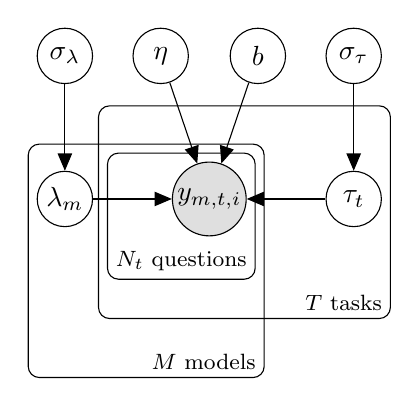
\begin{tikzpicture}
          % nodes
          \node[obs] (obs) {$y_{m,t, i}$};%

          \node[latent, right=of obs, xshift=0.0cm, yshift=-0.0cm] (task_difficulty) {\(\tau_{t}\)}; %

          \node[latent, left=of obs, xshift=0.0cm, yshift=0cm] (model_performance_across_task) {\( \lambda_{m}\)}; 


           \node[latent, above=of task_difficulty, yshift=0.1cm]  (task_difficulty_std) {$\sigma_\tau$ }; 

           \node[latent, above=of model_performance_across_task, yshift=0.0cm, yshift=0.1cm]  (model_performance_across_task_std) {$\sigma_\lambda$ }; 

           
          \node[latent, right=of model_performance_across_task_std, xshift=-0.5cm] (mass) {$\eta$}; 
          
          \node[latent, left=of task_difficulty_std, xshift=0.5cm] (bias) {$b$}; 
          
          % plates
          \coordinate (dummy_bottom) at ([yshift=-1.3cm] obs.south);
          \coordinate (dummy_top) at ([yshift=0.6cm] obs.north);
          \plate [inner sep=0.1cm] {platequestion} {(obs)
          } {$N_t$ questions}; 
          
          \plate [inner sep=0.1cm] {platetask} {
               (platequestion)  (task_difficulty) (dummy_top) % (acc)
          } {$T$ tasks}; 
          
          \plate [inner sep=0.1cm ] {platemodel} {
           (obs) (model_performance_across_task) (dummy_bottom) (platequestion)
          } {$M$ models}; 
          
          % edges
          \edge {task_difficulty, model_performance_across_task, bias, mass} {obs}
          \edge {task_difficulty_std} {task_difficulty}
          \edge {model_performance_across_task_std} {model_performance_across_task}
       
   \end{tikzpicture} 
    }
    \vspace{0.4em}
    \scriptsize Task-based model.
  \end{minipage}\hfill\pause
  \begin{minipage}[t]{0.32\textwidth}
    \centering
    \resizebox{\linewidth}{!}{%
      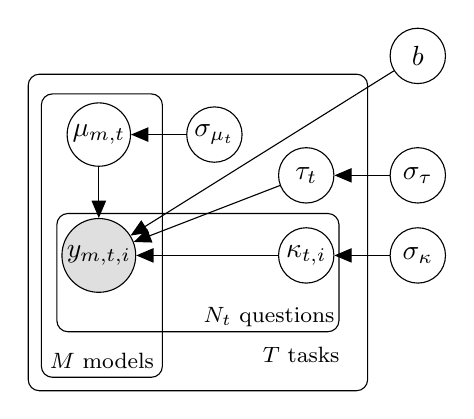
\begin{tikzpicture}
          % nodes
       
          %R
          \node[obs] (acc) {$y_{m,t, i}$};%
          %C
          \node[latent, right=of acc, xshift=0.8cm] (question_difficulty) { $\kappa_{t, i}$ };   
       
          %S
          \node[latent, above=of question_difficulty, xshift=0.0cm, yshift=-0.7cm] (task_difficulty) {\(\tau_{t}\)}; %
       
          \node[latent, above=of acc, xshift=0.0cm, yshift=-0.35cm] (model_performance_specific_task) {\( \mu_{m,t}\)}; 
          \node[latent, right=of model_performance_specific_task,xshift=-0.3cm]  (model_performance_specific_task_std) {\(\sigma_{\mu_t}\)}; %
           
          %global
          \node[latent, right=of question_difficulty, xshift=-0.3cm]  (question_difficulty_std) {$\sigma_\kappa$}; 
          \node[latent, right=of task_difficulty, xshift=-0.3cm]  (task_difficulty_std) {$\sigma_\tau$ }; 
          % Move beta to the global latents
          \node[latent, above=of task_difficulty_std, yshift=-0.2cm] (bias) {$b$}; 
                 
          
          % plates
          % \coordinate (dummy_bottom) at ([xshift=-0.9, yshift=-0.58cm] acc.south);
          \coordinate (dummy_temp) at ([yshift=-0.58cm] acc.south);
          \coordinate (dummy_bottom) at ([xshift=0.7cm] dummy_temp);
          \plate [inner sep=0.10cm ] {platemodel} {(acc) (model_performance_specific_task) (dummy_bottom)} {$M$ models}; 
          \plate [inner sep=0.05cm] {platequestion} {(acc)(question_difficulty)} {$N_t$ questions}; 
          \plate [inner sep=0.35cm] {platetask} {(platequestion)(task_difficulty)(model_performance_specific_task)(model_performance_specific_task_std)} {$T$ tasks}; 
       
          % edges
          \edge {bias, task_difficulty, question_difficulty, model_performance_specific_task} {acc}
          \edge {question_difficulty_std} {question_difficulty}
          \edge {task_difficulty_std} {task_difficulty}
          \edge {model_performance_specific_task_std} {model_performance_specific_task}
       
       \end{tikzpicture} 
    }
    \vspace{0.4em}
    \scriptsize Question-task difficulty model.
  \end{minipage}\hfill
  \pause
  \begin{minipage}[t]{0.32\textwidth}
    \centering
    \resizebox{\linewidth}{!}{%
     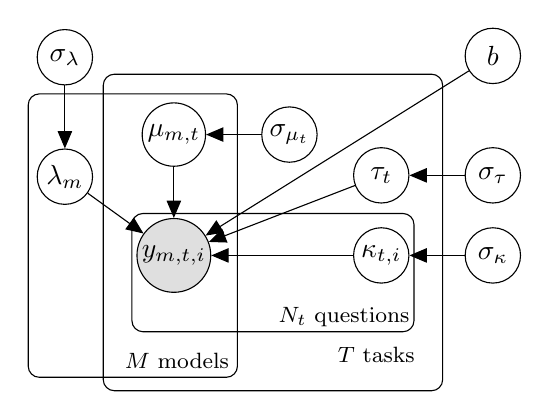
\begin{tikzpicture}
      % nodes

      %R
      \node[obs] (acc) {$y_{m,t, i}$};%
      %C
      \node[latent, right=of acc, xshift=0.8cm] (question_difficulty) { $\kappa_{t, i}$ };   

      %S
      \node[latent, above=of question_difficulty, xshift=0.0cm, yshift=-0.7cm] (task_difficulty) {\(\tau_{t}\)}; %

      \node[latent, above=of acc, xshift=0.0cm, yshift=-0.35cm] (model_performance_specific_task) {\( \mu_{m,t}\)}; 

      \node[latent, left=of acc, xshift=0.45cm, yshift=1.0cm] (model_performance_across_task) {\( \lambda_{m}\)}; 
      
      \node[latent, right=of model_performance_specific_task,xshift=-0.3cm]  (model_performance_specific_task_std) {\(\sigma_{\mu_t}\)}; %
       
      %global
      \node[latent, right=of question_difficulty, xshift=-0.3cm]  (question_difficulty_std) {$\sigma_\kappa$}; 
      \node[latent, right=of task_difficulty,xshift=-0.3cm]  (task_difficulty_std) {$\sigma_\tau$ }; 
      \node[latent, above=of model_performance_across_task, yshift=-0.2cm]  (model_performance_across_task_std) {$\sigma_\lambda$ }; 
      
      % Move beta to the global latents
      \node[latent, above=of task_difficulty_std, yshift=-0.2cm] (bias) {$b$}; 
             
      
      % plates
      % \coordinate (dummy_bottom) at ([yshift=-0.6cm] acc.south);
      \coordinate (dummy_temp) at ([yshift=-0.58cm] acc.south);
      \coordinate (dummy_bottom) at ([xshift=0.7cm] dummy_temp);
      \plate [inner sep=0.10cm ] {platemodel} {(acc) (model_performance_specific_task)  (model_performance_across_task)(dummy_bottom)} {$M$ models}; 
      \plate [inner sep=0.05cm] {platequestion} {(acc)(question_difficulty)} {$N_t$ questions}; 
      \plate [inner sep=0.35cm] {platetask} {(platequestion)(task_difficulty)(model_performance_specific_task)(model_performance_specific_task_std)} {$T$ tasks}; 

      % edges
      \edge {bias, task_difficulty, question_difficulty, model_performance_specific_task, model_performance_across_task} {acc}
      \edge {question_difficulty_std} {question_difficulty}
      \edge {task_difficulty_std} {task_difficulty}
      \edge {model_performance_specific_task_std} {model_performance_specific_task}
      \edge {model_performance_across_task_std} {model_performance_across_task}

   \end{tikzpicture}
    }
    \vspace{0.4em}
    \scriptsize + Across-task performance latent variable.
  \end{minipage}
  \par\vspace{0.8em}\small Graphical models of the proposed hierarchical models. \alert{Way too complicated!}
  
\end{frame}

\begin{frame}{Bayesian Evals for Interpretability}
  \begin{figure}
  \includegraphics[width=\textwidth, height=0.8\textheight, keepaspectratio]{img/bayes_evals/pretrained2.png}
  \end{figure}
  \pause 
  So just use Beta-Binomial!
\end{frame}




\begin{frame}{Future Directions}
  \begin{itemize}[<+->]
    \item If we make our latent variables for `model performance' and `benchmark difficulty' multivariate and sparse, maybe we can interpret their dimensions as different measures of model capability?
    \begin{itemize}
      \item E.g. one dimension is `physics knowledge', another is `reasoning ability' etc.
    \end{itemize}
    \item The results for this were interesting, but not as straightforwardly interpretable as we hoped.
    \item Perhaps these techniques could be used more successfully for predicting eval performance based on the mix of pretraining data?
    \item Or predicting the effectiveness of post-training on downstream evals?
  \end{itemize}
\end{frame}

\begin{frame}{Thank You}
  \begin{itemize}[<+->]
    \item Any questions?
  \end{itemize}
\end{frame}


\begin{frame}[allowframebreaks]{References}
  \nocite{*}
  \printbibliography
\end{frame}


\begin{frame}{IID Questions Setting: Prior Mismatch}
  Use $\theta \sim \text{Uniform}[0, 1]$ as the prior, but $\theta \sim \text{Beta}(100, 20)$ as the true data distribution. ($\mathbb{E}[\theta] = 0.83$ and $\text{Var}(\theta) = 0.034^2$.)
  \begin{figure}
      \includegraphics[width=\textwidth, height=0.75\textheight, keepaspectratio]{img/bayes_evals/fig/exp4-1_beta-100-20_mismatch.pdf}
      % \caption{Simulation results comparing Coverage and Width for different $N$.}
  \end{figure}
\end{frame}

\begin{frame}{Bayesian Evals for Interpretability}
  \begin{itemize}[<+->]
    \item Given eval questions and reponses, use an SAE-like model to enforce sparsity on features across the latent dimensions of `model performance' and `benchmark difficulty' vectors.
  \end{itemize}
  \vspace{-0.2cm}
  \pause
  \begin{figure}
    \includegraphics[width=\textwidth, height=0.77\textheight, keepaspectratio]{img/bayes_evals/fig/task_based_capabilities_IRT_capabilities_3.pdf}
  \end{figure}
\end{frame}


\begin{frame}{Clustered Questions Setting: Bayesian Implementation}
  \begin{figure}
    \includegraphics[width=\textwidth, height=0.8\textheight, keepaspectratio]{img/bayes_evals/bayes_evals_code3.png}
  \end{figure}
\end{frame}

\end{document}"
  % latex -jobname "handout-01" "\def\uselecture{01}\PassOptionsToClass{handout}{beamer}\documentclass[aspectratio=169]{beamer}
% \documentclass[aspectratio=169, handout]{beamer}

\usetheme{Madrid}
\usecolortheme{beaver}

\usepackage{graphicx}
\usepackage{amsmath}
\usepackage{amssymb}
\usepackage{amsthm}
\usepackage{mathrsfs}
\usepackage{hyperref}

\usepackage{tikz}
\usetikzlibrary{bayesnet}
\usetikzlibrary{arrows}


% \usepackage{graphicx}
% \usepackage{booktabs}
% \usepackage{pgfplots}
% \pgfplotsset{compat=1.14}
% \usepackage{anyfontsize}
% % \usepackage{minted}
% \usepackage[cache=false]{minted} 
% \setminted[python]{
%     linenos,
%     % bgcolor=LightGray,
%     % breaklines,
%     fontsize=\scriptsize,
%     % xleftmargin=1.1em,
%     numbersep=4pt
% }

% \usepackage{tcolorbox}

% \newtcolorbox[auto counter]{pbox}[2][]{
%   colback=white,
%   title=#2,
%   #1,
%   fonttitle= \large, %\sffamily,
%   % fontupper=\sffamily,
%   boxrule=0.5pt, 
%   arc=2pt,
%   top=1pt, 
%   bottom=1pt,
%   before={\vspace{2pt}}, 
%   after={\vspace{2pt}} 
%   % colframe=..,
%   % coltitle=..,
%   % colbacktitle=..,
%   % toptitle=0.05cm,
%   % bottomtitle=0.125cm
% }

% \usepackage{fancyvrb}


\setbeamertemplate{caption}{%
  \raggedright
  \insertcaption\par
}

\usepackage[style=authoryear, autocite=footnote, backend=biber]{biblatex}
\addbibresource{refs.bib}

\title[Cohere Research Talk]{Cohere Research Talk: Massively Parallel Inference \& Bayesian Evals}
\author{Sam Bowyer}
\date{November 2025}

\begin{document}

\begin{frame}
  \titlepage
\end{frame}

\begin{frame}{Outline}
  \tableofcontents
\end{frame}

% --- Part 1: Overview ---
\section{About Me}

\begin{frame}{About Me}
  \begin{itemize}[<+->] 
    \item Fourth (final) year PhD student at Bristol's Compass CDT (Computational Statistics and Data Science).
    \item Based in the School of Maths, but supervised by Laurence Aitchison (CS/Engineering Maths), Mengyue Yang (Engineering Maths), and Song Liu (Maths).
    \item Currently working on discrete diffusion models (training an `auxilliary' model with VI to suggest the order in which to decode tokens).
    % \item Also worked on RL and LoRA finetuning.
    \item Two projects I'll be talking about today: Alan (massively parallel probabilistic programming) \& Bayesian Evals.
  \end{itemize}
\end{frame}


% --- Part 2: Alan, Massively Parallel Inference ---
\section{Alan: Massively Parallel Probabilistic Programming}


\begin{frame}{Alan: A Massively Parallel Probabilistic Programming Language}
  \begin{figure}
    \centering
    \includegraphics[height=0.25\textheight]{img/laurence.png}
    \includegraphics[height=0.25\textheight]{img/thomas.png}
    \includegraphics[height=0.25\textheight]{img/sam.png}
    \caption{Work done with Laurence Aitchison and Thomas Heap over the first two years of my PhD.}
  \end{figure}
  \pause
  \begin{itemize}[<+->]
    % \item Work with Laurence Aitchison and Thomas Heap over the first two years of my PhD.
    \item Dual goals:
      \begin{itemize}
        \item Develop `massively parallel' Bayesian inference algorithms: fast, accurate, and scalable; desinged for GPU acceleration.
        \item Implement these algorithms in a probabilistic programming language in pytorch (\texttt{alan}), allowing users to specify general probabilistic models.
      \end{itemize}
  \end{itemize}
\end{frame}


\begin{frame}{Regular Bayesian Inference}
  \begin{itemize}[<+->]
    \item \textbf{Bayesian inference}: Prior $P(z)$ and likelihood $P(x|z)$ for latent variables $z$ and data $x$.
      $$P(z|x) = \frac{P(x|z)P(z)}{\int_\mathcal{Z} P(x,z') dz'}$$
    \item \textbf{Importance sampling}: 
      \begin{enumerate}
        \item Sample $K$ latent variables from a proposal distribution $Q$ (usually IID):
          $$z = (z^1, \ldots, z^K) \sim Q(z).$$ 
        \item Compute importance weights: 
          $$r_k(z) = \frac{P(x , z^k)}{Q(z^k)}.$$ 
        \item Approximate the normalising constant using the `global' estimator: 
          $$\mathcal{P}_\text{global}(z) = \frac{1}{K} \sum_{k=1}^K r_k(z) \quad \text{such that } \quad \mathbb{E}_{z \sim Q}[\mathcal{P}_\text{global}(z)] = P(x).$$ 
      \end{enumerate}
  \end{itemize}
\end{frame}

\begin{frame}{Limitations of Importance Sampling (IS)}
  \begin{itemize}[<+->]
    \item Global IS scales poorly with the number of latent variables, $n$.
    \begin{itemize}
      \item $z^k = (z_1^k, \ldots, z_n^k) \in \mathcal{Z}$.
      % \item E.g. $n$ is the dimension of $z$ if all latent variables are scalar.
    \end{itemize} 
    \item Chatterjee \& Diaconis (2018) show that as $n$ increases, the number of samples, $K$, must increase with $O(e^{D_{\text{KL}}(P(z|x) || Q(z))}) \approx O(e^n)$. (This is a lot!)
    \item Solution: \textbf{Massively Parallel Importance Sampling (MP-IS)}
      \begin{itemize}
        \item Reason about all $K^n$ possible joint samples at once.
      \end{itemize}
  \end{itemize}
\end{frame}


\begin{frame}{Massively Parallel Importance Sampling (MP-IS)}
  \begin{minipage}{0.55\textwidth}
    \begin{figure}
      \includegraphics[width=\textwidth]{img/alan/MPIS.pdf}
    \end{figure}
  \end{minipage}
  \begin{minipage}{0.43\textwidth}
    \begin{itemize}[<+->]
      \item Suppose each latent sample $z^k = (z_1^k, \ldots, z_n^k) \sim Q(z)$ is comprised of $n$ variables.
      \item We can construct $K^n$ different samples from the full joint space 
      $$(z_1^{k_1}, \ldots, z_n^{k_n}) \in \mathcal{Z}$$
      where $\mathbf{k} = (k_1, \ldots, k_n) \in [K]^n$ is the indexing vector for each latent variable.
    \end{itemize}
  \end{minipage}
\end{frame}

\begin{frame}{Massively Parallel Importance Sampling (MP-IS)}
  \begin{minipage}{0.55\textwidth}
    \begin{figure}
      \includegraphics[width=\textwidth]{img/alan/MPIS.pdf}
    \end{figure}
  \end{minipage}
  \begin{minipage}{0.43\textwidth}
    \begin{itemize}[<+->]
      \item Rather than using the global IS estimator
      $$\mathcal{P}_\text{global}(z) = \frac{1}{K} \sum_{k=1}^K \frac{P(x, z^k)}{Q(z^k)}.$$
      \item ...we can use the MP-IS estimator
      $$\mathcal{P}_\text{MP}(z) = \frac{1}{K^n} \sum_{\mathbf{k}\in [K]^n} \frac{P(x, z^\mathbf{k})}{Q_\text{MP}(z^\mathbf{k}, \mathbf{k})}.$$
      (Which is still unbiased.)
    \end{itemize}
  \end{minipage}
\end{frame}

% \begin{frame}{MP-IS: Some Complications...}
%   $$\mathcal{P}_\text{MP}(z) = \frac{1}{K^n} \sum_{\mathbf{k}\in [K]^n} \frac{P(x, z^\mathbf{k})}{Q_\text{MP}(z^\mathbf{k}, \mathbf{k})}.$$
%   \begin{itemize}[<+->]
%     \item We have to be careful about how we define $Q_\text{MP}$ over the space of all $K^n$ joint samples.
%     \item We can use a hierarchical model:
%       $$Q_\text{MP}(z, \mathbf{k}) = \prod_{i=1}^n Q_\text{MP}(z_i^{k_i} | z_j \text{ for } j \in \text{qa}(i)),$$
%       where $\text{qa}(i)$ is the set of indices of parents of $z_i$ in the proposal model.
%     \item If variable $z_i$ has a parent samples $z_j = (z_j^1, \ldots, z_j^K) \sim Q(z_j)$, then we can sample $z_i^{k_i}$ from $Q(z_i^{k_i} | z_j^{\pi(k_i)})$ for a (uniformly) random permutation $\pi$ of $[K]$.  \end{itemize}
% \end{frame}

\begin{frame}{MP-IS: Some Complications...}
  $$\mathcal{P}_\text{MP}(z) = \frac{1}{K^n} \sum_{\mathbf{k}\in [K]^n} \frac{P(x, z^\mathbf{k})}{Q_\text{MP}(z^\mathbf{k}, \mathbf{k})} = \frac{1}{K^n} \sum_{\mathbf{k}\in [K]^n} r_\mathbf{k}(z).$$

  \begin{itemize}[<+->]
    \item We have to be careful about how we define $Q_\text{MP}$ over the space of all $K^n$ joint samples.
    \item Also, at first glance, this thing doesn't look all that nice to compute...
    \item But we can exploit the conditional independencies in the model to render it tractable.
  \end{itemize}

\end{frame}


\begin{frame}{MP-IS: Some Complications...}

  \begin{figure}
    \includegraphics[width=0.6\textwidth]{img/alan/toy_model.drawio.pdf}
  \end{figure}

  \begin{itemize}[<+->]
    \item E.g. with the model from before with $n=3$, $P(x, z) =  P(z_1) P(z_2 | z_1) P(z_3 | z_2) P(x | z_3)$, we can move the sums inside the product and get a bunch of tensor products:
  \end{itemize}
    \pause
    $$
    % \begin{aligned}
      \mathcal{P}_\text{MP}(z) = \frac{1}{K^3} \sum_{k_1 \in [K]} \sum_{k_2 \in [K]} \sum_{k_3 \in [K]} \frac{P(z_1^{k_1}) P(z_2^{k_2} | z_1^{k_1}) P(z_3^{k_3} | z_2^{k_2}) P(x | z_3^{k_3})}{Q(z_1^{k_1}) Q(z_2^{k_2}) Q(z_3^{k_3})}
      % = \frac{1}{K^3} \sum_{k_1 \in [K]} \sum_{k_2 \in [K]} \sum_{k_3 \in [K]} r_{k_1,k_2,k_3}(z)
    $$
    \pause
    $$
      = \frac{1}{K^3} \sum_{k_1 \in [K]} \underbrace{\frac{P(z_1^{k_1})}{Q(z_1^{k_1})}}_{\text{Vector of size } K} 
      \sum_{k_2 \in [K]} \underbrace{\frac{P(z_2^{k_2} | z_1^{k_1})}{Q(z_2^{k_2})}}_{\text{Matrix of size } K \times K}
      \sum_{k_3 \in [K]} \underbrace{\frac{P(z_3^{k_3} | z_2^{k_2})}{Q(z_3^{k_3})}}_{\text{Matrix of size } K \times K}
      \underbrace{P(x | z_3^{k_3})}_{\text{Vector of size } K}
    % \end{aligned}
    $$
    % \item This can be computed efficiently on a GPU using tensor operations.
  % \end{itemize}
\end{frame}


\begin{frame}{Can we hide these complications from the user?}
  \begin{itemize}[<+->]
    \item Yes! We do this with \texttt{alan}.
    \item User specifies the model with P and Q as pytorch modules, and we handle the massively parallel inference for them.
  \end{itemize}
\end{frame}

\begin{frame}{Alan: A Probabilistic Programming Language}

  \begin{minipage}{0.7\textwidth}
    \begin{figure}
      \centering
      \includegraphics[width=0.9\textwidth]{img/alan/movielens_code_1.png}
    \end{figure}
  \end{minipage}
  \begin{minipage}{0.25\textwidth}
    % \vspace{-1cm}
    \begin{figure}[t]
      \centering
      \resizebox{0.8\textwidth}{!}{%
        \tikz{
          % nodes
           \node[obs] (rating) {\(\mathrm{Rating}_{mn}\)};%
           \node[latent,above=of rating] (peruser) {\(\mathbf{z}_m\)}; %
           \node[latent, above=of peruser, xshift=-1cm] (psi) {\(\boldsymbol{\psi}\)};
          \node[latent, above=of peruser, xshift=1cm] (mu) {\(\boldsymbol{\mu}\)};
          % plate
           \plate [inner sep=.3cm] {plate2} {(rating)} {\(\mathrm{N}\) Films}; %
           \plate [inner sep=.3cm] {plate1} {(peruser)(plate2)} {\(\mathrm{M}\) Users}; %
          edges
           \edge {psi,mu} {peruser}
           \edge {peruser} {rating}}
           }
    \end{figure}
  \end{minipage}

\end{frame}

\begin{frame}{MP-VI}
  \begin{itemize}[<+->]
    \item Using $\mathcal{P}_\text{MP}(z)$, we can do variational inference (VI) by maximising the ELBO:
      $$
      \log P(x) \geq \mathcal{L}_\text{MP}(\theta) = \mathbb{E}_{z \sim Q_\text{MP}(\theta)}[\log \mathcal{P}_\text{MP}(z)]
      $$
    \item Aitchison (2019) showed that MP-VI is a tighter bound than the global VI objective (IWAE):
      $$
      \log P(x) \geq \mathcal{L}_\text{MP}(\theta) \geq \mathcal{L}_\text{global}(\theta) = \mathbb{E}_{z \sim Q(\theta)}[\log \mathcal{P}_\text{global}(z)]
      $$
  \end{itemize}
  \pause
  \begin{figure}
    \centering
    \includegraphics[width=0.9\textwidth]{img/alan/movielens_code_2.png}
  \end{figure}
\end{frame}

\begin{frame}{MP Algorithms}
  \begin{itemize}[<+->]
    \item We can obtain unbiased posterior moment estimates via autodiff (Bowyer et al. (2024)).
      $$
      m_\text{MP}(z) = \frac{1}{K^n} \sum_{\mathbf{k} \in [K]^n} \frac{r_\mathbf{k}(z)}{\mathcal{P}_\text{MP}(z)}m(z^\mathbf{k})
      $$
    \item We define a modified marginal likelihood estimator with an auxiliary variable $J \in \mathbb{R}$:
      $$
      \mathcal{P}_\text{MP}^\text{exp}(z, J) = \frac{1}{K^n} \sum_{\mathbf{k} \in [K]^n} r_\mathbf{k}(z) \exp(J m(z^\mathbf{k}))
      $$
    \item Then differentiating the log of this with respect to $J$ and setting $J=0$ we get:
      $$
      \frac{\partial}{\partial J}\bigg|_{J=0} \log \mathcal{P}_\text{MP}^\text{exp} (z, J) = \frac{\frac{\partial}{\partial J}\bigg|_{J=0} \mathcal{P}_\text{MP}^\text{exp} (z, J)}{\mathcal{P}_\text{MP}^\text{exp} (z, 0)} = m_\text{MP}(z)
      $$
    \item By similar arguments: $J \in \mathbb{R}^K$ gives us marginal importance weights; $J \in \mathbb{R}^{K^{1+|pa(i)|}}$ gives us importance samples for $z_i$, given its parents $pa(i)$.
  \end{itemize}
  \vspace{0.1cm}
\end{frame}

\begin{frame}{QEM: An Adaptive Importance Sampling Algorithm}
  \begin{minipage}{0.4\textwidth}
    \textbf{QEM} (Heap et al. (2025))
    \begin{enumerate}
      \item Start with an initial approximate posterior $Q_0$.
      \item Compute posterior moment estimates $m_\text{MP}(z)$ using MP-IS.
      \item Update the approximate posterior $Q_{t+1}$ using the moment estimates.
    \end{enumerate}    
  
    Can be seen as an EM-like algorithm for adaptive imortance sampling.
  \end{minipage}
  \begin{minipage}{0.59\textwidth}
    \begin{figure}
      \centering
      \includegraphics[width=0.95\textwidth]{img/alan/QEM_results.pdf}
    \end{figure}
  \end{minipage}
\end{frame}

\begin{frame}{Conclusions}
  \begin{itemize}[<+->]
    \item This project was a great (if, at times, complicated) way to learn about Bayesian inference and numerical and probabilistic programming.
    \item The results were pretty promising, but but there are some drawbacks to massively parallel methods:
    \begin{itemize}
      \item The algorithms are complex to implement (hence wrapping them in a PPL).
      \item Not all models have lots of conditional independencies to exploit.
      \item Although it's slower and harder to tune, HMC is often hard to beat in terms of quality of inference.
    \end{itemize}
  \end{itemize}
\end{frame}

% --- Part 3: Bayesian Evals, Uncertainty Quantification for LLM Evals ---
\section{Bayesian Evals: Uncertainty Quantification for LLM Evals}

\begin{frame}{Bayesian Evals: Uncertainty Quantification for LLM Evals}
  \begin{figure}
    \centering
    \includegraphics[height=0.25\textheight]{img/laurence.png}
    \includegraphics[height=0.25\textheight]{img/desi.jpg}
    \includegraphics[height=0.25\textheight]{img/sam.png}
    \caption{Work done with Laurence Aitchison and Desi R. Ivanova.}
  \end{figure}
  \begin{itemize}[<+->]
    \item Two directions:
      \begin{itemize}
        \item Improved UQ for evals with Bayesian methods.
        \item Interpretability of evals with Bayesian hierarchical modelling and SAE-like approaches.
      \end{itemize}
    \item The former direction led to an ICML spotlight position paper: \emph{`Position: Don't Use the CLT in LLM Evals With Fewer Than a Few Hundred Datapoints'}.
    \item The latter fell by the wayside, but is something I'd like to come back to at some point.
  \end{itemize}
\end{frame}

% --- Slide 2: Motivation ---
\begin{frame}{Motivation}
  \begin{block}{Central Limit Theorem (CLT)}
    If $X_1, \dots, X_N$ are IID r.v.s with mean $\mu \in \mathbb{R}$ and finite variance $\sigma^2$, then 
    $$
      \sqrt{N} (\hat{\mu} - \mu) \xrightarrow{d} \mathcal{N}( 0, \sigma^2 ) \; \text{as } N \rightarrow \infty,
    $$
    where $\hat{\mu} = \frac{1}{N}\sum_{i=1}^N X_i$ is the sample mean.
  \end{block}
  \pause
  \begin{itemize}[<+->]
      % \item Error bars are important for interpreting evals.
      \item The CLT-based confidence interval is:
      $$
        \text{CI}_{1-\alpha}(\mu) = \hat{\mu} \pm z_{\alpha/2} \text{SE}(\hat{\mu})
      $$
      where $z_{\alpha/2}$ is the $100(1-\alpha/2)$-th percentile of $\mathcal{N}(0, 1)$ and $\text{SE}(\hat{\mu}) = \sqrt{\frac{\hat{\sigma}^2}{N}}$ is the standard error of the sample mean.
      \item In the case of binary data $X_i \in \{0, 1\}$, this becomes:
      $$
        \text{CI}_{1-\alpha}(\theta) = \bar{X} \pm z_{\alpha/2} \sqrt{\bar{X}(1-\bar{X})/N}.
      $$
  \end{itemize}
  
\end{frame}

\begin{frame}{Real-World Failures of the CLT}
  \begin{itemize}[<+->]
    \item If $N$ is too small, CLT-based error bars can collapse to \alert{zero-width} or \alert{extend past $[0,1]$}.
    \item Smaller, more intricate, and expensive LLM benchmarks are becoming increasingly common, so we need to find alternatives for the few-data regime.
  \end{itemize}
  % \vspace{0.5cm}
  \begin{minipage}{0.45\textwidth}
    \centering
    \begin{figure}
      \includegraphics[height=4.2cm, keepaspectratio]{img/bayes_evals/pngs/real_data_matharena_aime_II_subset.png}
      \caption{Math Arena's AIME II 2025 Benchmark (N=15). Various 95\% interval types shown.}
    \end{figure}
  \end{minipage}
  \begin{minipage}{0.45\textwidth}
    \centering
    \begin{figure}
        \includegraphics[height=4.2cm, keepaspectratio]{img/bayes_evals/langchain_clt.png}
        \caption{Langchain Typewriter Tool Use Benchmark (N=20). CLT-based 95\% intervals only.}
    \end{figure}
  \end{minipage}
\end{frame}

% --- Slide 3: Bayesian Alternative -- Beta-Bernoulli Model ---
\begin{frame}{Bayesian Alternative: Beta-Binomial Model}
  \begin{itemize}[<+->]
    \item Treat the data as IID Bernoulli with a \alert{uniform prior} on the parameter $\theta$.
    $$
      \begin{aligned}
      \theta &\sim \text{Beta}(1, 1) = \text{Uniform}[0, 1] \\
      y_i &\sim \text{Bernoulli}(\theta) \; \text{for } i=1,\dots N 
      \end{aligned}
    $$
    \item Say $y_i$ is correct if $y_i = 1$ and incorrect if $y_i = 0$. %(Think of $\theta$ as the probability of correctness.)  
    \item Obtain quantile-based Bayesian \alert{credible intervals} for $\theta$ from the closed form posterior.
    $$
      p(\theta | y_{1:N}) = \text{Beta}\left(1+\sum_{i=1}^N y_i, 1 + \sum_{i=1}^N (1-y_i)\right)
    $$

  \end{itemize}
  
\pause
\begin{figure}
  \centering
  \includegraphics[width=0.8\textwidth]{img/bayes_evals/bayes_evals_code1.png}
\end{figure}


% \begin{pbox}[label={ex:bayes_simple}]{Beta-Bernoulli Bayesian Credible Interval}
%   \begin{minted}[fontsize=\scriptsize,breaklines]{python}
%  y is a length N binary "eval" vector
% S, N = y.sum(), len(y)  total successes & questions

% # Bayesian Credible interval
% posterior = scipy.stats.beta(1 + sum(y), 1 + N - sum(y))
% bayes_ci  = posterior.interval(confidence=0.95)
%   \end{minted}
% \end{pbox}

\end{frame}

% --- Slide 4: Frequentist Alternatives ---
\begin{frame}{Frequentist Alternatives}
  % \vspace{1cm}
  \begin{itemize}[<+->]
      \item \alert{Wilson score interval}: Based on normal approximation to the binomial distribution.
        \pause
        $$ \text{CI}_{1-\alpha, \text{Wilson}}(\theta) = \frac{\hat{\theta} + \frac{z_{\alpha/2}^2}{2N}}{1 + \frac{z_{\alpha/2}^2}{N}} \pm \frac{\frac{z_{\alpha/2}}{2N}}{1 + \frac{z_{\alpha/2}^2}{N}}\sqrt{4N\hat{\theta}(1 - \hat{\theta}) + z_{\alpha/2}^2} $$
        \pause
      \item \alert{Clopper-Pearson `exact' interval}: A `worst-case' approach; very conservative method guaranteed to never under-cover.
      $\text{CI}_{1-\alpha, \text{CP}}(\theta) = [\theta_\text{lower}, \theta_\text{upper}]$, 
        \pause
        $$ \theta_\text{lower} = B\left(\frac{\alpha}{2}, \sum_{i=1}^N y_i, 1+\sum_{i=1}^N(1-y_i)\right) \; \text{and} \; \theta_\text{upper} = B\left(1-\frac{\alpha}{2}, 1+ \sum_{i=1}^N y_i, \sum_{i=1}^N(1-y_i)\right) $$
        where $B(\alpha, a, b)$ is the $\alpha$-th quantile of the Beta$(a, b)$ distribution.
  \end{itemize}
  
  \pause
  % \vspace{1cm}
  % Implementation using \texttt{scipy}:
%   \begin{verbatim}
% # y is a length N binary "eval" vector
% S, N = y.sum(), len(y) # total successes & questions
% result = scipy.stats.binomtest(k=S, n=N)

% # 95% Wilson score interval and Clopper-Pearson exact interval
% wilson_ci = result.proportion_ci("wilson", 0.95)
% cp_ci = result.proportion_ci("exact", 0.95)
%   \end{verbatim}
\begin{figure}
  \centering
  \includegraphics[width=0.8\textwidth]{img/bayes_evals/bayes_evals_code2.png}
\end{figure}
\end{frame}

% --- Slide 5: Interval Comparison Simulations ---
\begin{frame}{Interval Comparison Simulations}
  \vspace{1cm}
  We use synthetic eval data so that we \alert{know} the true parameter $\theta$.
  
  \begin{itemize}[<+->]
      \item Draw $\theta \sim \text{Uniform}[0, 1]$.
      \item Draw $N \in \{3,10,30,100\}$ IID Bernoulli datapoints with parameter $\theta$.
      \item Construct intervals with various methods for various $1-\alpha$ confidence levels.
      \item Repeat many times and calculate the true coverage and average width of the intervals.
      \begin{itemize}
        \item Coverage: What proportion of the time does a $1-\alpha$ confidence-level interval \alert{actually contain} the true parameter? (A frequentist metric, really.)
        \item Ideally, $\text{coverage} = 1-\alpha$.
      \end{itemize}
  \end{itemize}
\end{frame}

% --- Slide 6: IID Questions Setting ---
\begin{frame}{IID Questions Setting: Results}
  \begin{figure}
      \includegraphics[width=\textwidth, height=0.8\textheight, keepaspectratio]{img/bayes_evals/fig/exp4-1_top_row_only.pdf}
      % \caption{Simulation results comparing Coverage and Width for different $N$.}
  \end{figure}
\end{frame}

\begin{frame}{IID Questions Setting: Results}
  \begin{figure}
      \includegraphics[width=\textwidth, height=0.8\textheight, keepaspectratio]{img/bayes_evals/fig/exp4-1_inkscape.pdf}
      % \caption{Simulation results comparing Coverage and Width for different $N$.}
  \end{figure}
\end{frame}

% --- Slide 7: Other Eval Settings ---
\begin{frame}{Other Eval Settings}
  \begin{itemize}[<+->]
      \item \textbf{Clustered Questions}
      \begin{itemize}
          \item Instead of $N$ IID questions, we have $T$ tasks, each with $N_t$ IID questions.
      \end{itemize}
      
      \item \textbf{Comparisons Between Two Models, $\theta_A$ and $\theta_B$}
      \begin{itemize}
          \item Independent Comparisons (using $N_A, N_B, \bar{y}_A, \bar{y}_B$ only).
          \item Paired Comparisons (using $N_A = N_B, \{y_{A;i}\}_{i=1}^N, \{y_{B;i}\}_{i=1}^N$).
          % \item Hypothesis testing $H_0: \theta_A = \theta_B$ vs $H_1: \theta_A > \theta_B$.
          \item With Bayes you can calculate $\mathbb{P}(\theta_A > \theta_B | y_A, y_B)$.
      \end{itemize}
      
      \item \textbf{Metrics that aren't simple averages of binary results} (e.g. F1 score).
      
      \item \textbf{Prior Mismatch} (i.e. what if the uniform prior is incorrect, $\theta \nsim \text{Uniform}[0, 1]$?).
  \end{itemize}
\end{frame}


% --- Slide 8: Clustered Questions Setting ---
\begin{frame}{Clustered Questions Setting: Frequentist Approach}
  \begin{itemize}[<+->]
    \item Instead of $N$ IID questions, we have $T$ tasks, each with $N_t$ IID questions.
    \item Some tasks are easier than others.% (e.g. each task asks $N_t$ questions about a single piece of input text, with texts varying in difficulty).
    \item Frequentist approach (Miller, 2024):
    $$
    \text{CI}_{1-\alpha}(\theta) = \bar{X} \pm z_{\alpha/2} \text{SE}_\text{Clustered}
    $$
    $$
    \text{SE}_\text{Clustered} = \sqrt{\text{SE}_\text{CLT}^2 + \frac{1}{N^2}\sum_{t=1}^T \sum_{i=1}^{N_t} \sum_{j \neq i} (y_{i,t} - \bar{y})(y_{j,t} - \bar{y})}
    $$
    % \item An improved standard error, but fundamentally still using the CLT.
  \end{itemize}
\end{frame}


\begin{frame}{Clustered Questions Setting: A Bayesian Approach}
  \begin{itemize}[<+->]
    \item `Dispersion' parameter $d$ controls the range of difficulty across tasks,
    $$d \sim \text{Gamma}(1, 1).$$
    \item $\theta$ is the mean difficulty of the questions across tasks,
    $$
    \theta \sim \text{Beta}(1, 1) = \text{Uniform}[0, 1].
    $$
    \item $\theta_t$ is the difficulty of the questions in task $t$ (we ensure that $\mathbb{E}[\theta_t | \theta] = \theta$),
    $$  
    \theta_t \sim \text{Beta}(d \theta, d (1-\theta)).
    $$
    \item $\text{Var}(\theta_t | \theta) = \frac{\theta (1-\theta)}{d^2 + 1}$.
    \item If $d$ is large, then $\theta_t$ is close to $\theta$ for all tasks.
    \item If $d$ is small, then $\theta_t$ is more variable across tasks.
  \end{itemize}
\end{frame}

\begin{frame}{Clustered Questions Setting: A Bayesian Approach}
  \vspace{-0.5cm}
  $$
    \begin{aligned}
    d &\sim \text{Gamma}(1, 1), \quad 
    \theta \sim \text{Beta}(1, 1), \quad 
    \theta_t &\sim \text{Beta}(d \theta, d (1-\theta)), \quad
    y_{i,t} \sim \text{Bernoulli}(\theta_t)
    \end{aligned}
  $$
  \vspace{-0.5cm}
  \pause
  \begin{itemize}[<+->]
    \item Can we integrate out the per-task difficulty parameters $\theta_t$?
    \item Yes! The number of successes per task is \alert{Beta-Binomial} distributed: 
      $$
        \sum_{i=1}^{N_t} y_{i,t} = Y_t \sim \text{BetaBinomial}(N_t, d \theta, d (1-\theta)).
      $$
    \item Get an \alert{importance-weighted posterior} for $\theta$: draw prior samples $\{(\theta^{(k)}, d^{(k)})\}_{k=1}^K$, then compute weights
      $$
        w^{(k)} = \prod_{t=1}^T p(Y_t | \theta^{(k)}, d^{(k)}).
      $$
    \item Compute quantile-based Bayesian credible intervals for $\theta$.
  \end{itemize}
\end{frame}

\begin{frame}{Clustered Questions Setting: Results}
  \begin{figure}
      \includegraphics[width=\textwidth, height=0.8\textheight, keepaspectratio]{img/bayes_evals/pngs/exp4-2.png}
      % \caption{Simulation results comparing Coverage and Width for different $N$.}
  \end{figure}
\end{frame}


% --- Slide 9: Conclusion ---
\begin{frame}{Conclusion}
  Advice to practitioners:
  
  \begin{itemize}[<+->]
      \item Use \alert{Bayesian Beta-Bernoulli} or \alert{Wilson Score intervals} for IID setting.
      \item Use simple \alert{Bayesian models} for other settings (for flexibility and interpretability).
      \item It's \textbf{easy} (use \texttt{scipy} or \texttt{bayes\_evals}).
      \item It's \textbf{safer} than CLT-based methods.
      \item It's still \textbf{cheap} for large $N$.
  \end{itemize}
  
  \vspace{1cm}

  \pause
  My takeaways from this project:
  \begin{itemize}[<+->]
    \item The project really cemented my understanding of Bayesianism vs Frequentism in practice.
    \item There's a big communication gap between AI researchers and classical statisticians.
    \item UQ for evals is an incredibly rich space.
  \end{itemize}
  % \begin{columns}
  %     \column{0.5\textwidth}
  %     \centering
  %     \textbf{Paper} \\
  %     \href{https://arxiv.org/pdf/2503.01747}{https://arxiv.org/pdf/2503.01747} \\
  %     \vspace{0.5cm}
  %     \includegraphics[width=3cm]{img/bayes_evals/arxiv_qr.png}
      
  %     \column{0.5\textwidth}
  %     \centering
  %     \textbf{\texttt{bayes\_evals} package} \\
  %     \href{https://github.com/sambowyer/bayes_evals}{https://github.com/sambowyer/bayes\_evals} \\
  %     \vspace{0.5cm}
  %     \includegraphics[width=3cm]{img/bayes_evals/github_qr.png}
  % \end{columns}
\end{frame}


\begin{frame}{Bayesian Evals for Interpretability}
  \begin{itemize}[<+->]
    \item Apply hierarchical Bayesian modelling to evals: infer latent variables for \alert{benchmark difficulty} and \alert{model performance}.
  \end{itemize}

  \pause
  
  \begin{minipage}[t]{0.32\textwidth}
    \centering
    \resizebox{\linewidth}{!}{%
      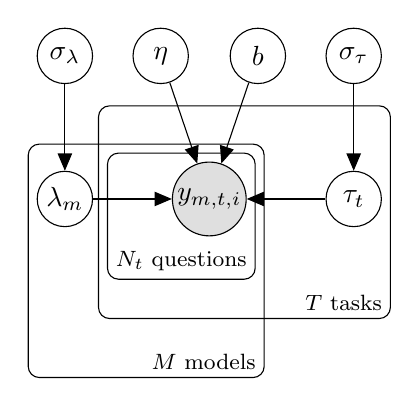
\begin{tikzpicture}
          % nodes
          \node[obs] (obs) {$y_{m,t, i}$};%

          \node[latent, right=of obs, xshift=0.0cm, yshift=-0.0cm] (task_difficulty) {\(\tau_{t}\)}; %

          \node[latent, left=of obs, xshift=0.0cm, yshift=0cm] (model_performance_across_task) {\( \lambda_{m}\)}; 


           \node[latent, above=of task_difficulty, yshift=0.1cm]  (task_difficulty_std) {$\sigma_\tau$ }; 

           \node[latent, above=of model_performance_across_task, yshift=0.0cm, yshift=0.1cm]  (model_performance_across_task_std) {$\sigma_\lambda$ }; 

           
          \node[latent, right=of model_performance_across_task_std, xshift=-0.5cm] (mass) {$\eta$}; 
          
          \node[latent, left=of task_difficulty_std, xshift=0.5cm] (bias) {$b$}; 
          
          % plates
          \coordinate (dummy_bottom) at ([yshift=-1.3cm] obs.south);
          \coordinate (dummy_top) at ([yshift=0.6cm] obs.north);
          \plate [inner sep=0.1cm] {platequestion} {(obs)
          } {$N_t$ questions}; 
          
          \plate [inner sep=0.1cm] {platetask} {
               (platequestion)  (task_difficulty) (dummy_top) % (acc)
          } {$T$ tasks}; 
          
          \plate [inner sep=0.1cm ] {platemodel} {
           (obs) (model_performance_across_task) (dummy_bottom) (platequestion)
          } {$M$ models}; 
          
          % edges
          \edge {task_difficulty, model_performance_across_task, bias, mass} {obs}
          \edge {task_difficulty_std} {task_difficulty}
          \edge {model_performance_across_task_std} {model_performance_across_task}
       
   \end{tikzpicture} 
    }
    \vspace{0.4em}
    \scriptsize Task-based model.
  \end{minipage}\hfill\pause
  \begin{minipage}[t]{0.32\textwidth}
    \centering
    \resizebox{\linewidth}{!}{%
      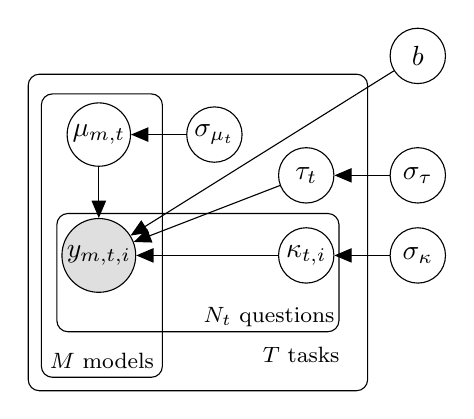
\begin{tikzpicture}
          % nodes
       
          %R
          \node[obs] (acc) {$y_{m,t, i}$};%
          %C
          \node[latent, right=of acc, xshift=0.8cm] (question_difficulty) { $\kappa_{t, i}$ };   
       
          %S
          \node[latent, above=of question_difficulty, xshift=0.0cm, yshift=-0.7cm] (task_difficulty) {\(\tau_{t}\)}; %
       
          \node[latent, above=of acc, xshift=0.0cm, yshift=-0.35cm] (model_performance_specific_task) {\( \mu_{m,t}\)}; 
          \node[latent, right=of model_performance_specific_task,xshift=-0.3cm]  (model_performance_specific_task_std) {\(\sigma_{\mu_t}\)}; %
           
          %global
          \node[latent, right=of question_difficulty, xshift=-0.3cm]  (question_difficulty_std) {$\sigma_\kappa$}; 
          \node[latent, right=of task_difficulty, xshift=-0.3cm]  (task_difficulty_std) {$\sigma_\tau$ }; 
          % Move beta to the global latents
          \node[latent, above=of task_difficulty_std, yshift=-0.2cm] (bias) {$b$}; 
                 
          
          % plates
          % \coordinate (dummy_bottom) at ([xshift=-0.9, yshift=-0.58cm] acc.south);
          \coordinate (dummy_temp) at ([yshift=-0.58cm] acc.south);
          \coordinate (dummy_bottom) at ([xshift=0.7cm] dummy_temp);
          \plate [inner sep=0.10cm ] {platemodel} {(acc) (model_performance_specific_task) (dummy_bottom)} {$M$ models}; 
          \plate [inner sep=0.05cm] {platequestion} {(acc)(question_difficulty)} {$N_t$ questions}; 
          \plate [inner sep=0.35cm] {platetask} {(platequestion)(task_difficulty)(model_performance_specific_task)(model_performance_specific_task_std)} {$T$ tasks}; 
       
          % edges
          \edge {bias, task_difficulty, question_difficulty, model_performance_specific_task} {acc}
          \edge {question_difficulty_std} {question_difficulty}
          \edge {task_difficulty_std} {task_difficulty}
          \edge {model_performance_specific_task_std} {model_performance_specific_task}
       
       \end{tikzpicture} 
    }
    \vspace{0.4em}
    \scriptsize Question-task difficulty model.
  \end{minipage}\hfill
  \pause
  \begin{minipage}[t]{0.32\textwidth}
    \centering
    \resizebox{\linewidth}{!}{%
     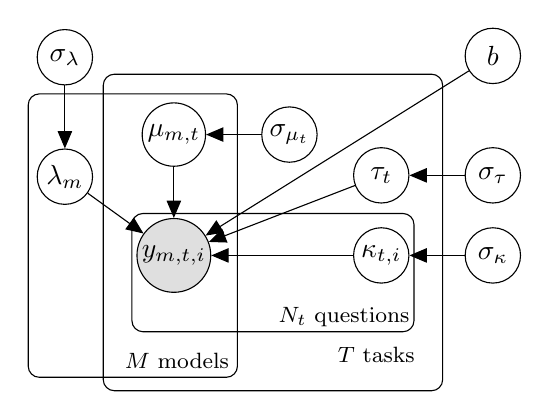
\begin{tikzpicture}
      % nodes

      %R
      \node[obs] (acc) {$y_{m,t, i}$};%
      %C
      \node[latent, right=of acc, xshift=0.8cm] (question_difficulty) { $\kappa_{t, i}$ };   

      %S
      \node[latent, above=of question_difficulty, xshift=0.0cm, yshift=-0.7cm] (task_difficulty) {\(\tau_{t}\)}; %

      \node[latent, above=of acc, xshift=0.0cm, yshift=-0.35cm] (model_performance_specific_task) {\( \mu_{m,t}\)}; 

      \node[latent, left=of acc, xshift=0.45cm, yshift=1.0cm] (model_performance_across_task) {\( \lambda_{m}\)}; 
      
      \node[latent, right=of model_performance_specific_task,xshift=-0.3cm]  (model_performance_specific_task_std) {\(\sigma_{\mu_t}\)}; %
       
      %global
      \node[latent, right=of question_difficulty, xshift=-0.3cm]  (question_difficulty_std) {$\sigma_\kappa$}; 
      \node[latent, right=of task_difficulty,xshift=-0.3cm]  (task_difficulty_std) {$\sigma_\tau$ }; 
      \node[latent, above=of model_performance_across_task, yshift=-0.2cm]  (model_performance_across_task_std) {$\sigma_\lambda$ }; 
      
      % Move beta to the global latents
      \node[latent, above=of task_difficulty_std, yshift=-0.2cm] (bias) {$b$}; 
             
      
      % plates
      % \coordinate (dummy_bottom) at ([yshift=-0.6cm] acc.south);
      \coordinate (dummy_temp) at ([yshift=-0.58cm] acc.south);
      \coordinate (dummy_bottom) at ([xshift=0.7cm] dummy_temp);
      \plate [inner sep=0.10cm ] {platemodel} {(acc) (model_performance_specific_task)  (model_performance_across_task)(dummy_bottom)} {$M$ models}; 
      \plate [inner sep=0.05cm] {platequestion} {(acc)(question_difficulty)} {$N_t$ questions}; 
      \plate [inner sep=0.35cm] {platetask} {(platequestion)(task_difficulty)(model_performance_specific_task)(model_performance_specific_task_std)} {$T$ tasks}; 

      % edges
      \edge {bias, task_difficulty, question_difficulty, model_performance_specific_task, model_performance_across_task} {acc}
      \edge {question_difficulty_std} {question_difficulty}
      \edge {task_difficulty_std} {task_difficulty}
      \edge {model_performance_specific_task_std} {model_performance_specific_task}
      \edge {model_performance_across_task_std} {model_performance_across_task}

   \end{tikzpicture}
    }
    \vspace{0.4em}
    \scriptsize + Across-task performance latent variable.
  \end{minipage}
  \par\vspace{0.8em}\small Graphical models of the proposed hierarchical models. \alert{Way too complicated!}
  
\end{frame}

\begin{frame}{Bayesian Evals for Interpretability}
  \begin{figure}
  \includegraphics[width=\textwidth, height=0.8\textheight, keepaspectratio]{img/bayes_evals/pretrained2.png}
  \end{figure}
  \pause 
  So just use Beta-Binomial!
\end{frame}




\begin{frame}{Future Directions}
  \begin{itemize}[<+->]
    \item If we make our latent variables for `model performance' and `benchmark difficulty' multivariate and sparse, maybe we can interpret their dimensions as different measures of model capability?
    \begin{itemize}
      \item E.g. one dimension is `physics knowledge', another is `reasoning ability' etc.
    \end{itemize}
    \item The results for this were interesting, but not as straightforwardly interpretable as we hoped.
    \item Perhaps these techniques could be used more successfully for predicting eval performance based on the mix of pretraining data?
    \item Or predicting the effectiveness of post-training on downstream evals?
  \end{itemize}
\end{frame}

\begin{frame}{Thank You}
  \begin{itemize}[<+->]
    \item Any questions?
  \end{itemize}
\end{frame}


\begin{frame}[allowframebreaks]{References}
  \nocite{*}
  \printbibliography
\end{frame}


\begin{frame}{IID Questions Setting: Prior Mismatch}
  Use $\theta \sim \text{Uniform}[0, 1]$ as the prior, but $\theta \sim \text{Beta}(100, 20)$ as the true data distribution. ($\mathbb{E}[\theta] = 0.83$ and $\text{Var}(\theta) = 0.034^2$.)
  \begin{figure}
      \includegraphics[width=\textwidth, height=0.75\textheight, keepaspectratio]{img/bayes_evals/fig/exp4-1_beta-100-20_mismatch.pdf}
      % \caption{Simulation results comparing Coverage and Width for different $N$.}
  \end{figure}
\end{frame}

\begin{frame}{Bayesian Evals for Interpretability}
  \begin{itemize}[<+->]
    \item Given eval questions and reponses, use an SAE-like model to enforce sparsity on features across the latent dimensions of `model performance' and `benchmark difficulty' vectors.
  \end{itemize}
  \vspace{-0.2cm}
  \pause
  \begin{figure}
    \includegraphics[width=\textwidth, height=0.77\textheight, keepaspectratio]{img/bayes_evals/fig/task_based_capabilities_IRT_capabilities_3.pdf}
  \end{figure}
\end{frame}


\begin{frame}{Clustered Questions Setting: Bayesian Implementation}
  \begin{figure}
    \includegraphics[width=\textwidth, height=0.8\textheight, keepaspectratio]{img/bayes_evals/bayes_evals_code3.png}
  \end{figure}
\end{frame}

\end{document}"
  \expandafter\includeonlylecture\expandafter{\uselecture}
\else
  % Default lecture to output - comment out to get all lectures
  \includeonlylecture{01}
\fi

% Uncomment to get title slides for each lecture
% \AtBeginLecture{
%   \subtitle{\insertlecture}
%   \setcounter{framenumber}{0}
%   \begin{frame}
%     \titlepage
%   \end{frame}
% }

%%%%%%%%%%%%%%%%%%%%%%%%%%%%%%%%%%%%%%%%%%%%%%%%%%%%%%%%%%%%%%%%%%%%%%%%%%%%%%
% Start of the slides

\begin{document}

% Available frame options:
%   leftcolor, rightcolor: set the colour of the left or right panel
%   leftimage, rightimage: put a (cropped) image in the left or right panel
%   div: set the location of the divider between left and right panels
%   urlcolor: set the colour of the url

% Other commands available:
%   \logo{X}: choose the logo to display (logo, white logo, or black logo)
%   \urltext{X}: change the url for each slide

% All standard University of Bristol colours are available:
%   UniversityRed, CoolGrey, BrightAqua, BrightBlue, BrightOrange, BrightPurple,
%   BrightPink, BrightLime, DarkAqua, DarkBlue, DarkOrange, DarkPurple,
%   DarkPink, DarkLime

\begin{frame}[leftcolor=white,rightcolor=UniversityRed,div=0.8\paperwidth]
  \titlepage
\end{frame}

%%%%%%%%%%%%%%%%%%%%%%%%%%%%%%%%%%%%%%%%%%%%%%%%%%%%%%%%%%%%%%%%%%%%%%%%%%%%%%
\lecture{Lecture 1}{01}

\begin{frame}
\frametitle{Table of Contents}
\tableofcontents
\end{frame}

\section{1. Recap: Spectral Clustering}
%%%%%%%%%%%%%%%%%%%%%%%%%%%%%%%%%%%%%%%%%%%%%%%%%%%%%%%%%%%%
\begin{frame}{Basic Spectral Clustering Algorithm}
    To cluster $n$ data points $\{\mathbf{x}_i\}_{i=1}^n$ into $K$ clusters:
    \begin{enumerate}[<+->]
      \item Form the affinity/similarity matrix $W \in \mathbb{R}^{n \times n}$ where $W_{ij} = \exp\left(-\frac{d^2(\mathbf{x}_i, \mathbf{x}_j)}{\sigma^2}\right)$ for $i \neq j$ and $W_{ii} = 0$.
      \item Let $G$ be the diagonal matrix with $G_{ii} = \sum_{j=1}^n W_{ij}$ (the degree of $x_i$).
      Let $\tilde{L} \vcentcolon = G^{-1/2} W G^{-1/2}$ be the symmetric normalized Laplacian.
      \item Form the matrix $Z \in \mathbb{R}^{n \times K}$ by stacking the eigenvectors corresponding to the $K$ largest eigenvalues of $\tilde{L}$.
      % \item Re-normalise the rows of $Z$ to unit length, giving $Z' \in \mathbb{R}^{n \times K}$ where $Z_{ij}' = Z_{ij}/\left({\sum_{l=1}^K Z_{il}^2}\right)^{1/2}$.
      \item Cluster the rows of $Z$ using $K$-means: assign $x_i$ to cluster $k \in [K] \vcentcolon= \{1, \ldots, K\}$ if and only if row $i$ of $Z$ was assigned to cluster $k$.
    \end{enumerate}
    \cite{ng_spectral_2001}

\end{frame}

\section{2. Self-Tuning Spectral Algorithm}
%%%%%%%%%%%%%%%%%%%%%%%%%%%%%%%%%%%%%%%%%%%%%%%%%%%%%%%%%%%%
\begin{frame}{Parameters To Tune}
    \alert{Problem:} we have to choose $K$ and $\sigma$.
    \newline
    \pause

    \alert{Self-Tuning Spectral Clustering} \cite{zelnik-manor_self-tuning_2004} contributions:
    \begin{itemize}
      \item[(i)] Selection of the appropriate scale to analyse the data.
      \item[(ii)] Clustering data distributed at different scales.
      \item[(iii)] Clustering with irregular background clutter.
      \item[(iv)] Estimating the number of clusters.
    \end{itemize}
    \pause
    Selecting a suitable $\sigma$ will resolve (i)--(iii), whilst (iv) is just choosing $K$.
\end{frame}

\subsection{Selecting $\sigma$}
%%%%%%%%%%%%%%%%%%%%%%%%%%%%%%%%%%%%%%%%%%%%%%%%%%%%%%%%%%%%
\begin{frame}{Selecting $\sigma$}
    Note that $\sigma$ can be \alert{very} sensitive.
    \begin{figure}
      \centering
      \includegraphics[scale=0.3]{sensitive_sigma.png}
      \caption{Fig. 1 from \cite{zelnik-manor_self-tuning_2004}.}
    \end{figure}
\end{frame}

%%%%%%%%%%%%%%%%%%%%%%%%%%%%%%%%%%%%%%%%%%%%%%%%%%%%%%%%%%%%
\begin{frame}{Local Scaling}
    Furthermore, different bandwidths $\sigma$ may be needed for different clusters which are distributed at different scales.
    So we introduce \alert{local scaling}:
    \pause
    \begin{enumerate}%[<+->]
      \item For each data point $\mathbf{x}_i$, define $\sigma_i = d(x_i, x_P)$, i.e. the distance from $x_i$ to its $P$th nearest neighbour, $x_P$. ($P=7$ suggested.)
      \pause
      \item The \textit{locally scaled} affinity matrix's non-diagonal entries are given by $\hat{W}_{ij} = \exp\left(-\frac{d^2(x_i, x_j)}{\sigma_i \sigma_j}\right)$.
    \end{enumerate}
    \pause
    \begin{figure}
      \centering
      \includegraphics[scale=0.22]{local_scaling.png}
      \caption{Fig. 2 from \cite{zelnik-manor_self-tuning_2004}: (a) Input data; (b) unscaled affinity; (c) locally-scaled affinity (edge thickness represents weight).}
    \end{figure}
\end{frame}

\subsection{Selecting $K$}
%%%%%%%%%%%%%%%%%%%%%%%%%%%%%%%%%%%%%%%%%%%%%%%%%%%%%%%%%%%%
\begin{frame}{Selecting $K$}
    In the ideal case that there are some $K$ completely disconnected clusters (i.e. $\hat{W}_{ij} > 0$ if and only if $x_i$ and $x_j$ are in the same cluster), then the eigenvalues of $\tilde{L}$, given by $\lambda_1 \geq \lambda_2 \geq \cdots \geq \lambda_n$, will be such that:
    \[1 = \lambda_1 = \cdots = \lambda_K > \lambda_{K+1} \geq \cdots \geq \lambda_n \geq 0.\]
    
    This leads to the ``eigengap heuristic" for choosing $K$: choose $K$ to be the smallest integer such that $\lambda_{K} - \lambda_{K+1}$ is large.
    \newline\newline
    \pause
    However, with real, noisy data, the above may not hold (``lacks a theoretical justification" \cite{zelnik-manor_self-tuning_2004})---so instead of looking at the eigenvalues, we'll look further into the structure of $\tilde{L}$'s eigenvectors.

\end{frame}

%%%%%%%%%%%%%%%%%%%%%%%%%%%%%%%%%%%%%%%%%%%%%%%%%%%%%%%%%%%%
\begin{frame}{Analysing the Eigenvectors}
  In our ideal case (i.e. with $K$ completely disconnected clusters), $\tilde{L}$ is block diagonal, with each block $\tilde{L}^{(k)}$ corresponding to a cluster $k \in [K]$.
  \pause
  Therefore when we construct $Z \in \mathbb{R}^{n \times K}$ by stacking the eigenvectors of $\tilde{L}$ corresponding to the $K$ largest eigenvalues of $\tilde{L}$, we obtain
  \[Z = \begin{bmatrix}
    \mathbf{v}^{(1)} & \overrightarrow{\mathbf{0}} &\overrightarrow{\mathbf{0}} \\
    \overrightarrow{\mathbf{0}}  & \hdots &  \overrightarrow{\mathbf{0}} \\
    \overrightarrow{\mathbf{0}} & \overrightarrow{\mathbf{0}} & \mathbf{v}^{(K)}
  \end{bmatrix} \in \mathbb{R}^{n \times K}\]
  where $\mathbf{v}^{(k)}$ is the eigenvector corresponding to the largest eigenvalue (i.e. 1) of the submatrix $\tilde{L}^{(k)}$.
  
  % Each row $i$ of $Z$ has only one nonzero entry, lying in the column $j$ corresponding to $x_i$'s cluster.
  % Taking more than $K$ eigenvectors would result in more than one nonzero entry in some rows of $Z$, whilst taking fewer would result in some rows of $Z$ having no nonzero entries.

\end{frame}

%%%%%%%%%%%%%%%%%%%%%%%%%%%%%%%%%%%%%%%%%%%%%%%%%%%%%%%%%%%%
\begin{frame}{Analysing the Eigenvectors}
  % In our ideal case (i.e. with $K$ completely disconnected clusters), $\tilde{L}$ is block diagonal, with each block $\tilde{L}^{(k)}$ corresponding to a cluster $k \in [K] = \{1, \ldots, K\}$.
  % Therefore when we construct $Z \in \mathbb{R}^{n \times K}$ by stacking the eigenvectors of $\tilde{L}$ corresponding to the $K$ largest eigenvalues of $\tilde{L}$, we obtain
  \[Z = \begin{bmatrix}
    \mathbf{v}^{(1)} & \overrightarrow{\mathbf{0}} &\overrightarrow{\mathbf{0}} \\
    \overrightarrow{\mathbf{0}}  & \hdots &  \overrightarrow{\mathbf{0}} \\
    \overrightarrow{\mathbf{0}} & \overrightarrow{\mathbf{0}} & \mathbf{v}^{(K)}
  \end{bmatrix} \in \mathbb{R}^{n \times K}\]
  % where $\mathbf{v}^{(k)}$ is the eigenvector corresponding to the largest eigenvalue (i.e. 1) of the submatrix $\tilde{L}^{(k)}$.
  
  \begin{itemize}
    \item[1.] Each row $i$ of $Z$ has only one nonzero entry, lying in the column $j$ corresponding to $x_i$'s cluster---making the remaining task of cluster allocation trivial.
    \pause
    \item[2.] Taking more than $K$ eigenvectors would result in more than one nonzero entry in some rows of $Z$, whilst taking fewer would result in some rows of $Z$ having no nonzero entries.
  \end{itemize}
  \pause
  With noisy, non-ideal data the rows of $Z$ may have more than one nonzero entry, but there should hopefully be one entry significantly larger than the others.
  
  Assign $x_i$ to the cluster $k = \argmax_j Z_{ij}^2$.
\end{frame}

%%%%%%%%%%%%%%%%%%%%%%%%%%%%%%%%%%%%%%%%%%%%%%%%%%%%%%%%%%%%
\begin{frame}{A Problem With $Z$}
  % \newline\newline
  \alert{Problem:} The eigensolver we use may not return the $K$ eigenvectors of $\tilde{L}$ in the standard basis---it could return any set of orthonormal vectors spanning the same space as $Z$'s columns.
  \pause

  \alert{Solution:} Find the rotation matrix $R \in \mathbb{R}^{K \times K}$ that minimises the cost function
  \[J_K = \sum_{i=1}^n \sum_{j=1}^K \frac{\hat{Z}_{ij}^2}{\max_l (\hat{Z}_{il}^2)}\]
  where $\hat{Z} = Z R$ is the rotated matrix of eigenvectors.% and $M_i = \max_l \hat{Z}_{il}$.
  \pause
  \newline\newline
  Minimising this attempts to make the rows of $\hat{Z}$ as close to the standard basis as possible (i.e. with only one nonzero entry) and can be done via gradient descent (see \cite{zelnik-manor_self-tuning_2004} for details).
  
\end{frame}

%%%%%%%%%%%%%%%%%%%%%%%%%%%%%%%%%%%%%%%%%%%%%%%%%%%%%%%%%%%%
\begin{frame}{Selecting $K$ from $\hat{Z}$}
  Choosing some large $K'$ we can calculate the value of $J_K$ for all $K \in [K']$ efficiently as follows:
  \pause
  \begin{enumerate}
    \item Let $Z \in \mathbb{R}^{n \times 2}$ be the matrix of eigenvectors of $\tilde{L}$ corresponding to the two largest eigenvalues of $\tilde{L}$.
    \pause\item Find the rotation $R$ that minimises $J_K$ on $Z \in \mathbb{R}^{n \times 2}$ to obtain $\hat{Z}$.
    \pause\item Add the eigenvector corresponding to the next largest eigenvalue of $\tilde{L}$ as a column to $\hat{Z}$ and find the rotation $R$ that minimises $J_K$ for $K = 3$.
    \pause\item Repeat until we've found $J_{K'}$.
  \end{enumerate}
  \pause
  Finally, we choose $K_{\text{best}} = \argmin_{K \in [K']} J_K$.
  (Although, if several $K$s have very similar costs---e.g. within 0.01\% of each other---then choose the largest of these $K$s.)

  \end{frame}

%%%%%%%%%%%%%%%%%%%%%%%%%%%%%%%%%%%%%%%%%%%%%%%%%%%%%%%%%%%%
\begin{frame}{Cluster Allocation}
  Now that we have $K_{\text{best}}$, using the rotated matrix $\hat{Z} \in \mathbb{R}^{n \times K_{\text{best}}}$ we can allocate each data point $x_i$ to a cluster $k$ in one of two ways: 
  \pause 
  \begin{enumerate}[<+->]
    \item Assign $x_i$ to the cluster $k = \argmax_j \hat{Z}_{ij}^2$.
    \item As in the old algorithm, perform $K$-means on the rows of $\hat{Z}$ to find the clusters (this should converge fairly quickly since \alert{(1)} is likely to be a good initialisation).
    This is particularly useful for very noisy data.
  \end{enumerate}
\end{frame}

\subsection{Algorithm}
%%%%%%%%%%%%%%%%%%%%%%%%%%%%%%%%%%%%%%%%%%%%%%%%%%%%%%%%%%%%
\begin{frame}{Self-Tuning Spectral Clustering Algorithm}
  % To cluster $n$ data points $\{\mathbf{x}_i\}_{i=1}^n$:
  \begin{enumerate}[<+->]
    \item Compute the local scale $\sigma_i$ for each data point $x_i$.
    \item Form the locally scaled affinity matrix $\hat{W} \in \mathbb{R}^{n \times n}$ where $\hat{W}_{ij} = \exp\left(-\frac{d^2(\mathbf{x}_i, \mathbf{x}_j)}{\sigma_i \sigma_j}\right)$ for $i \neq j$ and $\hat{W}_{ii} = 0$. 
    \item Let $G$ be the diagonal matrix with $G_{ii} = \sum_{j=1}^n \hat{W}_{ij}$ (the degree of $x_i$) and $\tilde{L} \vcentcolon = G^{-1/2} \hat{W} G^{-1/2}$ be the symmetric normalized Laplacian.
    % \item Form the matrix $Y \in \mathbb{R}^{n \times K'}$ by stacking the eigenvectors of $\tilde{L}$ corresponding to the $K'$ largest eigenvalues of $\tilde{L}$ (for some large $K'$).
    \item For some large $K'$, form the matrix $Z \in \mathbb{R}^{n \times K'}$ by stacking the eigenvectors corresponding to the $K'$ largest eigenvalues of $\tilde{L}$ and use gradient descent to find the rotation matrix $R \in \mathbb{R}^{K' \times K'}$ that minimizes $J_{K'} = \sum_{i=1}^n \sum_{j=1}^{K'} (Z_{ij}^2 / \max_l Z_{il}^2)$. %M_i^2$ where $M_i = \max_j Z_i$.
    \item Choose $K_{\text{best}} = \argmin_K J_K$ (or largest such $K$ if several give very similar costs).
    \item Assign $x_i$ to cluster $k$ if and only if $\max_j Z_{ij}^2 = Z_{ik}^2$. 
    (Or, for very noisy data, use $K$-means to cluster the rows of $Z$ as in the standard algorithm.)
  \end{enumerate}
\cite{zelnik-manor_self-tuning_2004}
\end{frame}

\section{3. Experiments}
%%%%%%%%%%%%%%%%%%%%%%%%%%%%%%%%%%%%%%%%%%%%%%%%%%%%%%%%%%%%
\begin{frame}{}
    \begin{figure}
      \centering
      \includegraphics[width=0.8\textwidth]{code/regularSC.png}
      \caption{Iris dataset}
    \end{figure}
\end{frame}

%%%%%%%%%%%%%%%%%%%%%%%%%%%%%%%%%%%%%%%%%%%%%%%%%%%%%%%%%%%%
\begin{frame}{}
  \begin{figure}
    \centering
    \includegraphics[width=0.8\textwidth]{code/STSC.png}
    \caption{Iris dataset}
  \end{figure}
\end{frame}

%%%%%%%%%%%%%%%%%%%%%%%%%%%%%%%%%%%%%%%%%%%%%%%%%%%%%%%%%%%%
\begin{frame}{Conclusion}
    \begin{itemize}
      \item Self-tuning spectral clustering allows us to determine suitable values of $\sigma$ and $K$ automatically.
      \item We do have to choose $P$ and $K'$, but these are much simpler to tune (and we can usually just set $K'$ to be `big enough' in some sense).
      \item The local scaling implemented to deal with $\sigma$ also allows us to perform clustering noisy, multi-scale data.
    \end{itemize}
\end{frame}

%%%%%%%%%%%%%%%%%%%%%%%%%%%%%%%%%%%%%%%%%%%%%%%%%%%%%%%%%%%%
\begin{frame}{References}
        \bibliography{refs.bib}
\end{frame}

%%%%%%%%%%%%%%%%%%%%%%%%%%%%%%%%%%%%%%%%%%%%%%%%%%%%%%%%%%%%
\begin{frame}{Thank you}
\centering
    Any questions?
\end{frame}

% %%%%%%%%%%%%%%%%%%%%%%%%%%%%%%%%%%%%%%%%%%%%%%%%%%%%%%%%%%%%
% \begin{frame}{Using Gradient Descent To Find Eigenvalue Rotations}
%   bhk;vjhv
%   \end{frame}

\end{document}

%%%%%%%%%%%%%%%%%%%%%%%%%%%%%%%%%%%%%%%%%%%%%%%%%%%%%%%%%%%%%%%%%%%%%%%%%%%%%%
